%================================================================
% SLO
%----------------------------------------------------------------
% datoteka:     thesis_template.tex
%
% opis:         predloga za pisanje diplomskega dela v formatu LaTeX na
%               Univerza v Ljubljani, Fakulteti za računalništvo in informatiko
%
% pripravili:   Matej Kristan, Zoran Bosnić, Andrej Čopar,
%               po začetni predlogi Gašperja Fijavža
%
% popravil:     Domen Rački
%
% verzija:      1. april 2015
%================================================================
% ENG
%----------------------------------------------------------------
% file:         thesis_template.tex
%
% description:  template file for writing the diploma thesis in LaTeX format at
%               University of Ljubljana, Faculty of Computer and Information Science
%
% prepared by:  Matej Kristan, Zoran Bosnić, Andrej Čopar,
%               after the initial template from Gašper Fijavž
%
% edited by:    Domen Rački
%
% version:      1. april 2015
%================================================================





%================================================================
% SLO: definiraj strukturo dokumenta
% ENG: define file structure
%================================================================
\documentclass[a4paper, 12pt]{book}

%----------------------------------------------------------------
% |||||||||||||||||||||| USTREZNO POPRAVI |||||||||||||||||||||||
% |||||||||||||||||||||| EDIT ACCORDINGLY |||||||||||||||||||||||
%----------------------------------------------------------------
% SLO: definiraj metapodatke za datoteko thesis_template.tex
% ENG: define metadata for the file thesis_template.tex
%----------------------------------------------------------------
\usepackage{filecontents}
\begin{filecontents*}{\jobname.xmpdata}
    \Author{Gregor Majcen}
    \Title{Interaktivne računalniške umetniške instalacije v času hitrega tehnološkega razvoja}
    \Keywords{
        računalnik\sep
        umetnost\sep
        pametni telefon\sep
        android\sep
        filter\sep
        digitalna umetnost\sep
        ohranjanje\sep
        vzdrževanje programske opreme\sep
    }
    \Org{Univerza v Ljubljani, Fakulteta za računalništvo in informatiko}
\end{filecontents*}
% NOTE: the command \Subject is avoided in the given example since there are persisting problems with it
% NOTE: if you have errors conserning ICC profiles, read the pdfx package description file pdfx.pdf, section 'Color profiles'
%----------------------------------------------------------------
% |||||||||||||||||||||| USTREZNO POPRAVI |||||||||||||||||||||||
% |||||||||||||||||||||| EDIT ACCORDINGLY |||||||||||||||||||||||
%----------------------------------------------------------------

%================================================================
% SLO: vključi oblikovanje in pakete
% ENG: include design and packages
%================================================================
%----------------------------------------------------------------
% SLO: generiranje PDFjev iz pdftex, skladnih s PDF/A
% ENG: generating PDF/A compliant PDFs from pdftex
%----------------------------------------------------------------
\usepackage[a-1b]{pdfx}
%----------------------------------------------------------------
% SLO: LaTeX paketi
% ENG: LateX packages
%----------------------------------------------------------------
% SLO: omogoča uporabo slovenskih (latinskih) črk kodiranih v formatu UTF-8
% ENG: enables the use of slovene (latin) caracters encoded in the UFT-8 format
\usepackage[utf8x]{inputenc}   
% SLO: naloži, med drugim, slovenske delilne vzorce
% ENG: loads, among others, slovene dividing patterns
\usepackage[slovene,english]{babel} 
% SLO: poskrbi za postavitev strani
% ENG: takes care of the page layout
\usepackage{fancyhdr}
% SLO: za vlaganje slik različnih formatov
% ENG: for loading figures of different formats
\usepackage{graphicx}
\usepackage{caption}
\captionsetup[figure]{labelfont=bf} % SLO: napis "Slika #" v krepkem tisku
									% ENG: wirte "Figure #" caption in bold
\captionsetup[table]{labelfont=bf} % SLO: napis "Tabela #" v krepkem tisku
								   % ENG: wirte "Table #" caption in bold
% SLO: za pisanje psevdokode
% ENG: for writing pseudocode
\usepackage{algorithm}
\usepackage{algorithmic}
\floatname{algorithm}{\footnotesize Algorithm} % SLO: napis "Algoritem #" v krepkem tisku
											   % ENG: write "Algorithm #" caption in bold
% SLO: poveže reference slik/tabel in slike/tabele znotraj dokumenta
% ENG: links image/table references with the images/tables within the document
\usepackage{hyperref}
% SLO: pri kliku na referenco slike/tabele se postavi na vrh slike/tabele
% ENG: when clicking the image/table reference, position the focus on top of the image/table
\usepackage[all]{hypcap}
% SLO: omogoča, med drugim, definicjo in uporebo barve
% ENG: enables, among others, the definition and use of colors
\usepackage{xcolor}
%----------------------------------------------------------------
% SLO: dodatni paketi
% ENG: additional packages
%----------------------------------------------------------------
% SLO: omogoča večjo manipulacijo nad tabelami
% ENG: allows for greater manipulation of tables
\usepackage{booktabs}
% SLO: naloži dodatne simbole
% ENG: loads additional symbols
\usepackage{amssymb} 
% SLO: omogoča, med drugim, sklicevanje na formule z eqref
% ENG: enables, among others, equation referencing with eqref
\usepackage{amsmath}
% SLO: omogoča komentiranje večjega dela teksta
% ENG: enables the commenting of larger text parts
\usepackage{verbatim}
% SLO: omogoča rotacijo PDF strani v ležeč položaj
% ENG: enables the rotation of a PDF page to landscape
\usepackage{pdflscape}
% SLO: omogoča barvanje vrstic in stolpcev tabel
% ENG: enables coloring of table rows and columns
\usepackage{colortbl}



%================================================================
% SLO: nastavitve dokumenta
% ENG: document properties
%================================================================
% SLO: prilagoditev robov za tisk
% ENG: margin adjustments for printing
\addtolength{\marginparwidth}{-20pt}
\addtolength{\oddsidemargin}{40pt}
\addtolength{\evensidemargin}{-40pt}
% SLO: razmik med vrsticami
% ENG: line spacing
\renewcommand{\baselinestretch}{1.3} 
% SLO: postavitev strani
% ENG: page layout
\renewcommand{\chaptermark}[1]{\markboth{\MakeUppercase{\thechapter.\ #1}}{}} 
\renewcommand{\sectionmark}[1]{\markright{\MakeUppercase{\thesection.\ #1}}} 
\renewcommand{\headrulewidth}{0.5pt} % Header rule
\renewcommand{\footrulewidth}{0pt} % Footer rule
%
\fancypagestyle{frontmatter}{%
	\fancyhf{} % Clear all headers and footers first
	\fancyhead[LE,RO]{\sl \thepage} 
	%\fancyhead[LO]{\sl \rightmark} 
	%\fancyhead[RE]{\sl \leftmark}
}
\fancypagestyle{mainmatter}{%
  	\fancyhf{} % Clear all headers and footers first
	\fancyhead[LE,RO]{\sl \thepage} 
	\fancyhead[LO]{\sl \rightmark} 
	\fancyhead[RE]{\sl \leftmark}
}
% SLO: font za ime avtorja
% ENG: font for author name
\newcommand{\authorfont}{\Large}
% SLO: font za naslov diplomskega dela
% ENG: font for thesis title
\newcommand{\titlefont}{\LARGE\bf}
% SLO: globina kazala
% ENG: content depth
\setcounter{tocdepth}{1}
% SLO: definiraj ukaz za prazno stran
% ENG: define the command for empty page
\newcommand{\clearemptydoublepage}{\newpage{\pagestyle{empty}\cleardoublepage}}
\usepackage{listings}

\DeclareCaptionFont{white}{\color{white}}
\DeclareCaptionFormat{listing}{\colorbox{gray}{\parbox{\textwidth}{#1#2#3}}}
\captionsetup[lstlisting]{format=listing,labelfont=white,textfont=white}

\definecolor{forestgreen}{RGB}{34,139,34}
\definecolor{orangered}{RGB}{239,134,64}
\definecolor{darkblue}{rgb}{0.0,0.0,0.6}
\definecolor{gray}{rgb}{0.4,0.4,0.4}

\renewcommand{\lstlistingname}{Izsek}

\lstdefinestyle{java}{
    language=Java,
    aboveskip=3mm,
    belowskip=3mm,
    showstringspaces=false,
    columns=flexible,
    basicstyle={\footnotesize\ttfamily},
    breaklines=true,
    breakatwhitespace=true,
    tabsize=4
}

\lstdefinestyle{XML} {
    language=XML,
    extendedchars=true, 
    breaklines=true,
    breakatwhitespace=true,
    emph={},
    emphstyle=\color{red},
    basicstyle=\ttfamily,
    columns=fullflexible,
    commentstyle=\color{gray}\upshape,
    morestring=[b]",
    morecomment=[s]{<?}{?>},
    morecomment=[s][\color{forestgreen}]{<!--}{-->},
    keywordstyle=\color{orangered},
    stringstyle=\ttfamily\color{black}\normalfont,
    tagstyle=\color{black}\bf,
    morekeywords={attribute,xmlns,version,type,release},
    otherkeywords={attribute=, xmlns=},
}

\usepackage{subcaption}


%================================================================
% SLO: razno
% ENG: other
%================================================================
% SLO: nastavitev sklicevanj
% ENG: hyper referencing setup
\definecolor{black}{rgb}{0,0,0}
\hypersetup{
    colorlinks = true,
    linkcolor = black,
    citecolor = black,
    urlcolor = black
}
%----------------------------------------------------------------
% |||||||||||||||||||||| USTREZNO POPRAVI |||||||||||||||||||||||
% |||||||||||||||||||||| EDIT ACCORDINGLY |||||||||||||||||||||||
%----------------------------------------------------------------
\newcommand{\myname}{Gregor Majcen}
\newcommand{\mytitle}{Interaktivne računalniške umetniške instalacije v času hitrega tehnološkega razvoja}
\newcommand{\myyear}{2015}
\newcommand{\mysupervisor}{prof.~dr.\ Franc Solina}
%----------------------------------------------------------------
% SLO: dodaj poti do datotek s slikami, tabelami, ...
% ENG: add paths to files containing figures, tables, ...
%----------------------------------------------------------------
\graphicspath{
    {./figures/}
    {./tables/}
}
%----------------------------------------------------------------
% SLO: moji paketi
% ENG: my packages
%----------------------------------------------------------------
% ...
%----------------------------------------------------------------
% SLO: moji konstrukti
% ENG: my constructs
%----------------------------------------------------------------
\newtheorem{izrek}{Izrek}[chapter]
\newtheorem{trditev}{Trditev}[izrek]
\newenvironment{dokaz}{\emph{Dokaz.}\ }{\hspace{\fill}{$\Box$}}
\newcommand{\BibTeX}{{\sc Bib}\TeX}
%----------------------------------------------------------------
% |||||||||||||||||||||| USTREZNO POPRAVI |||||||||||||||||||||||
% |||||||||||||||||||||| EDIT ACCORDINGLY |||||||||||||||||||||||
%----------------------------------------------------------------





%================================================================
% SLO: začetne strani diplomskega dela
% ENG: fist pages of the diploma thesis
%================================================================
\begin{document}
% SLO: nastavi privzeti jezik
% ENG: set default language
\selectlanguage{slovene}
%\selectlanguage{english}

% SLO: prepreči težave s številkami strani v kazalu
% ENG: prevents problems with the page numbers in the contents page
\renewcommand{\thepage}{}

%----------------------------------------------------------------
% SLO: naslovnica (vstavi naslovnico (LaTeX kodo) iz datoteke pages/title.tex)
% ENG: title page (insert the title page (LaTeX code) from the file pages/title.tex)
%----------------------------------------------------------------
\thispagestyle{empty}
	\begin{center}
        {\large\sc Univerza v Ljubljani\\Fakulteta za računalništvo in informatiko}
    	\vskip 10em
    	{\authorfont \myname \par}
    	{\titlefont \mytitle \par}
    {\vskip 2em \textsc{MAGISTRSKO DELO\\[2mm]
    ŠTUDIJSKI PROGRAM DRUGE STOPNJE\\RAČUNALNIŠTVO IN INFORMATIKA}\par}
    \vfill\null
    {\large \textsc{Mentor}: \mysupervisor \par}
    {\vskip 2em \large Ljubljana, \myyear \par}
\end{center} \clearemptydoublepage
%\thispagestyle{empty}
	\begin{center}
        {\large\sc University of Ljubljana\\Faculty of Computer and Information Science}
    	\vskip 10em
    	{\authorfont \myname \par}
    	{\titlefont \mytitle \par}
    {\vskip 2em \textsc{MASTERS THESIS\\[2mm]
    THE 2nd CYCLE MASTERS STUDY PROGRAMME\\COMPUTER AND INFORMATION SCIENCE}\par}
    \vfill\null
    {\large \textsc{Supervisor}: \mysupervisor \par}
   	{\large \textsc{Co-supervisor}:  \mycosupervisor \par}
    {\vskip 2em \large Ljubljana, \myyear \par}
\end{center} \clearemptydoublepage

%----------------------------------------------------------------
% SLO: avtorske pravice
% ENG: copyright
%----------------------------------------------------------------
\thispagestyle{empty}
\vspace*{\fill}
{\noindent\footnotesize
{\sc Avtorske pravice}. Rezultati magistrskega dela so intelektualna lastnina avtorja in Fakultete za ra\-ču\-nal\-niš\-tvo in informatiko Univerze v Ljubljani. Za objavljanje ali izkoriščanje rezultatov ma\-gi\-str\-ske\-ga dela je potrebno pisno soglasje avtorja, Fakultete za ra\-ču\-nal\-niš\-tvo in informatiko ter mentorja.}
\begin{center}
{\footnotesize{\sc \copyright \myyear\ \myname}}
\end{center} \clearemptydoublepage
%\thispagestyle{empty}
\vspace*{\fill}
{\noindent\footnotesize
{\sc Copyright}. The results of this Masters Thesis are the intellectual property of the author and the Faculty of Computer and Information Science, University of Ljubljana. For the publication or exploitation of the Masters Thesis results, a written consent of the author, the Faculty of Computer and Information Science, and the supervisor is necessary.}
\begin{center}
{\footnotesize{\sc \copyright \myyear\ \myname}}
\end{center} \clearemptydoublepage

%----------------------------------------------------------------
% SLO: izjava o avtorstvu
% ENG: declaration of authorship
%----------------------------------------------------------------
\vspace*{1cm}
\begin{center}
{\Large \textbf{\sc Izjava o avtorstvu magistrskega dela}}
\end{center}

\vspace{1cm}
\noindent Spodaj podpisani \myname\ sem avtor magistrskega dela z naslovom:

\vspace{0.5cm}
\begin{center}
\emph{\mytitle}
\end{center}

\vspace{1cm}
\noindent S svojim podpisom zagotavljam, da:
\begin{itemize}
    \item sem magistrsko delo izdelal samostojno pod mentorstvom prof.~dr.\ Franca Soline,

    \item so elektronska oblika magistrskega dela, naslov (slovenski, angleški), povzetek (slovenski, angleški) ter ključne besede (slovenske, angleške) identični s tiskano obliko magistrskega dela,
    \item soglašam z javno objavo elektronske oblike magistrskega dela v zbirki ``Dela FRI''.
\end{itemize}

\vspace{1cm}
\noindent V Ljubljani, 13. avgusta 2015 \hfill Podpis avtorja:
 \clearemptydoublepage
%\vspace*{1cm}
\begin{center}
{\Large \textbf{\sc Declaration of Masters Thesis authorship}}
\end{center}

\vspace{1cm}
\noindent I, the undersigned \myname\ am the author of the Master Thesis entitled:

\vspace{0.5cm}
\begin{center}
\emph{\mytitle}
\end{center}

\vspace{1cm}
\noindent With my signature, I declare that:
\begin{itemize}
	\item the submitted Thesis is my own unaided work under the supervision of \mysupervisor\ and co-supervision of \mycosupervisor,

	\item all electronic forms of the Masters Thesis, title (Slovenian, English), abstract (Slovenian, English) and keywords (Slovenian, English) are identical to the printed form of the Masters Thesis,
	\item I agree with the publication of the electronic form of the Masters Thesis in the collection ''Dela FRI''. 
\end{itemize}

\vspace{1cm}
\noindent In Ljubljana, 3. April 2015 \hfill Author's signature: \clearemptydoublepage

%----------------------------------------------------------------
% SLO: zahvala
% ENG: acknowledgements
%----------------------------------------------------------------
\thispagestyle{empty}

\begin{center}
{\Large \textbf{\sc Zahvala}}
\end{center}
\vspace{0.5cm}

{\it\noindent
Hvala mentorju prof. dr. Francu Solini za vso strokovno pomoč in material za izdelavo magistrskega dela.

Hvala neuradnemu somentorju viš. pred. dr. Borutu Batagelju za pomoč tako pri izdelavi praktičnega dela magistrskega dela kot tudi pri dobavi strojne opreme.

Največja zahvala gre ženi Mateji za spodbudo, podporo in zabavo, ki je nastala med testiranjem praktičnega dela.

Hvala tudi moji in ženini družini za vso spodbudo, da zmorem.

Hvala prijatelju in sodelavcu Maticu Potočniku za komentarje, ideje in debate o tem, kaj vse bi se iz te naloge še dalo narediti.

Hvala tudi Teji, ki je to delo lektorirala, da branje lepše in lažje teče.

\vspace{0.5cm} \hfill \myname, \myyear
}
 \clearemptydoublepage
%\thispagestyle{empty}

\begin{center}
{\Large \textbf{\sc Acknowledgments}}
\end{center}
\vspace{0.5cm}

{\it\noindent
Worth mentioning in the acknowledgment is everyone who contributed to your thesis.

\vspace{0.5cm} \hfill \myname, \myyear
} \clearemptydoublepage

%----------------------------------------------------------------
% SLO: kazalo
% ENG: contents
%----------------------------------------------------------------
\begingroup
    \hypersetup{colorlinks=true,linkcolor=black}
    \def\thepage{}
    \tableofcontents{}
    \clearemptydoublepage
\endgroup

%----------------------------------------------------------------
% SLO: kratice
% ENG: abbreviations
%----------------------------------------------------------------
\chapter*{Seznam uporabljenih kratic}

\begin{tabular}{l|p{5cm}|p{6cm}}
  {\bf kratica} & {\bf angleško} & {\bf slovensko} \\ \hline
  % after \\: \hline or \cline{col1-col2} \cline{col3-col4} ...
  {\bf LCD} & Liquid crystal display & Zaslon s tekočimi kristali \\
  {\bf SIM} & Subscriber identity module & Identifikacijska kartica za storitve mobilne telefonije \\
  {\bf HDMI} & High-Definition Multimedia Interface & Vmesnik za prenašanje multimedijske vsebine v visoki ločljivosti \\
  {\bf API} & Application programming interface & Programski vmesnik \\
  {\bf SDK} & Software development kit & Komplet programskih orodij za razvijanje programske opreme \\
  {\bf JIT} & Just-in-time compilation & Dinamični prevajalnik, ki prevaja kodo med izvajanjem programa \\
  {\bf AOSP} & Android Open Source Project & Odprtokodni projekt Android \\
  {\bf JNI} & Java Native Interface & Izvorni javanski vmesnik \\
  {\bf OpenGL} & Open Graphics Library & Knjižnica za računalniško grafiko \\
  {\bf ES} & Embedded system & Namenski sistem \\
  {\bf GNU} & GNU's Not Unix! & Operacijski sistem, podoben Unixu, ki je sestavljen iz prostega programja \\
  {\bf GIMP} & GNU Image Manipulation Program & GNU program za predelovanje slik \\
  {\bf HSL} & Hue, saturation, lightness & Barvni odtenek, intenzivnost, svetlost
\end{tabular}
 \clearemptydoublepage
%\input{front_pages/eng/abbreviations} \clearemptydoublepage



%================================================================
% SLO: glavne strani diplomskega dela
% ENG: main pages of the diploma thesis
%================================================================
% SLO: izklopi številčenje poglavji in uporabi rimskime številkami za številke strani
% ENG: turns off chapter numbering and uses roman numerals for page numbers
\frontmatter
\pagestyle{frontmatter}



%---------------------------------------------------------------
% SLO: slovenski povzetek
% ENG: slovenian abstract
%---------------------------------------------------------------
\selectlanguage{slovene} % Preklopi na slovenski jezik
\chapter{Povzetek}

V okviru magistrske naloge je bila ponovno implementirana in nadgrajena
interaktivna umetniška instalacija ``15 sekund slave''. Motivacija za
instalacijo je umetniško delovanje ameriškega popart umetnika Andyja Warhola.
``15 sekund slave'' izgleda kot klasična slika, a je dejansko računalniški
zaslon, okvirjen kot umetniška slika. Nad zaslonom je v okviru vgrajen
digitalni fotoaparat, ki je povezan z računalnikom v ozadju. Vsakih petnajst
sekund fotoaparat slika obiskovalce galerije, ki stojijo pred sliko. Na sliki
računalniški program poišče vse obraze in nato naključno izbere enega izmed
njih. Ta obraz nato z grafičnimi filtri program obdela tako, da pridobi tako
imenovani popart videz z manjšim številom živih barv, ki spominjajo na
slike slavnih osebnosti, ki jih je iz fotografij delal Andy Warhol. Ker je
prvotna instalacija nastala pred več kot desetimi leti in se je strojna oprema v
tem času že zelo spremenila, se je pokazala potreba po prilagoditvi aplikacije
novemu stanju tehnologije. V nalogi so opisani problemi pri vzdrževanju
novomedijskih umetniških instalacij in kako smo le-te rešili v primeru opisane
instalacije.

\subsection*{Ključne besede}
\textit{računalnik, umetnost, pametni telefon, android, filter, digitalna umetnost, ohranjanje, vzdrževanje programske opreme}
\clearemptydoublepage



%---------------------------------------------------------------
% SLO: angleški povzetek
% ENG: english abstract
%---------------------------------------------------------------
\selectlanguage{english} % Preklopi na angleški jezik
\chapter{Abstract}

This thesis describes the reimplementation of the interactive art installation
entitled ``15 seconds of fame''. The motivation for the installation was the
famous American artist Andy Warhol. He modified simple photograph portraits
into pop-art pieces. The production of such portraits is the goal of the
installation ``15 seconds of fame''. The installation looks like a picture on
a wall, but it is in fact a computer monitor framed as a picture. On the top
of the frame there is a small camera which is connected to a computer hidden
behind the scene. Every fifteen seconds, the camera takes a picture of the
scene in front of it and sends it to the computer, where all the magic happens. It
searches for human faces in the picture, picks one face randomly and applies a
combination of image filters which converts the face into a pop-art
portrait. The idea is still great, even ten years later, but the original
technology is outdated and increasingly difficult to maintain. We reimplemented
the installation with new hardware and software and we discuss the problems of
maintaining new media art installations in general.

\subsection*{Keywords}
\textit{computer, art, smartphone, android, filter, digital art, conservation, software maintenance}
\clearemptydoublepage



\selectlanguage{slovene} % Preklopi na slovenski jezik
%================================================================
% SLO: osrednji del naloge
% ENG: main part of the paper
%================================================================
% SLO: vklopi številčenje poglavji, ponastavi številčenje strani in uporabi arabske številkami za številčenje strani
% ENG: turns on chapter numbering, resets page numbering and uses arabic numerals for page numbers
\mainmatter
\pagestyle{mainmatter}



\chapter{Uvod}
\newcommand{\refPoglavju}[1]{\ref{#1}.~poglavju}

Magistrska naloga sodi na relativno novo področje vzdrževanja novomedijskih
umetniških instalacij, ki za svoje delovanje potrebujejo računalniško
tehnologijo~\cite{firstdecade}. Umetniki so se za ta način ustvarjanja
odločili že kmalu po pojavu prvih računalnikov, vendar niso bili zadovoljni z
osnovnimi aplikacijami, saj so želeli pri svojih umetninah prikazati nekaj
več~\cite{miller2}. Tu pa se je pričelo sodelovanje z računalniškimi
strokovnjaki~\cite{miller1}.

V magistrski nalogi bomo posodobili interaktivno umetniško instalacijo ``15
sekund slave''. Najprej se bomo v \refPoglavju{ch:AndyWarhol_popart} seznanili
z motivacijo za to instalacijo in spoznali, kako instalacija deluje.

V \refPoglavju{ch:prvotnaIzvedba15} se seznanimo, kako je bila instalacija
prvotno implementirana.

Da bi se naloge pravilno lotili, smo v
\refPoglavju{ch:ohranjanjeDigitalneUmetnosti} preučili širšo problematiko
vzdrževanja novomedijskih umetniških del. Kako sploh vzdrževati umetniško
instalacijo, ki temelji na računalniški tehnologiji. Kakšni so principi in
strategije. Novejše v tem kontekstu ne pomeni vedno boljše. Zaradi hitrega
napredka računalniške tehnologije je potrebno take aplikacije po eni strani
prilagajati novi strojni in sistemski programski opremi, pa tudi novim
funkcionalnim možnostim, ki jih nove tehnologije nudijo. Po drugi strani pa z
umetniškega vidika običajno želimo, da se zunanja pojava umetniškega dela ne
spremeni.

V \refPoglavju{ch:nadgradnjaNaprava} smo po preučevanju teorije,
kako se sploh pravilno lotiti nadgradnje umetniške instalacije ``15 sekund
slave'', začeli razmišljati še s praktičnega vidika. V desetih letih, odkar
je bila prvotna instalacija narejena, je računalniška tehnologija močno
napredovala, še posebej v razvoju mobilnih naprav. Razmišljali smo, kako bi
novo tehnologijo lahko prenesli v trenutno instalacijo. Odločili smo se za
mobilni telefon. Pametni telefoni so enostavno in prosto dostopni na trgu in
ker se masovno izdelujejo, tudi niso zelo dragi. Vsebujejo pa vse, kar
potrebujemo: kamero, prikaz slike in programabilnost. Ostale lastnosti so le
bonus. Sedaj je bilo potrebno izbrati le še operacijski sistem. Zaradi osebnih
izkušenj smo se odločili za operacijski sistem Android~(\ref{sec:android}). Po
izbiri strojne opremo smo začeli z načrtovanjem, kako prenesti vso obstoječo
programsko funkcionalnost.

V \refPoglavju{ch:zaznavanjeObrazov} smo se soočili z zaznavanjem obrazov.
Načini, kako zaznavati obraze na sliki, so se v desetih letih močno
spreminjali. Obstaja tudi že veliko orodij, ki nam pomagajo pri tem. Naša
izbira je na koncu pristala na dveh orodjih:
OpenCV~(\ref{sec:zaznavanjeObrazovOpenCV}) in
AndroidSDK~(\ref{sec:zaznavanjeObrazovAndroidSDK}). Ti dve orodji temeljita na
popolnoma različnih strategijah, zato smo se odločili poskusiti obe.

V \refPoglavju{ch:obdelavaSlik} smo obravnavali obdelavo slik. Že pri prvotni
instalaciji je bilo izhodišče za vse filtre programsko orodje
GIMP~(\ref{sec:obdelavaSlikGIMP}). V tej instalaciji smo se odločili, da si
bomo tudi pomagali s tem programskim orodjem, vendar z različico iz današnjega
časa. Iz programskega orodja GIMP smo si izbrali tri vrste filtrov:
\begin{itemize}
    \item uravnovešanje barv~(\ref{sec:obdelavaSlikUravnovesanjeBarv}),
    \item posteriziranje~(\ref{sec:obdelavaSlikPosteriziranje}),
    \item uravnovešanje barv v prostoru HSL~(\ref{sec:obdelavaSlikUravnovesanjeBarvHSL}).
\end{itemize}
Različni parametri in mešanje teh filtrov med seboj so nas pripeljali do
popart slik~(\ref{sec:obdelavaSlikSestavljanjePopArt}).

S tem je bila prestavitev iz originalnega sistema v mobilni sistem končana.
Vendar pa smo želeli še več. V \refPoglavju{ch:novosti} opisujemo nove
funkcionalne možnosti, ki smo jih dodali za popestritev instalacije.

V \refPoglavju{ch:socialNetwork} pa smo se ukvarjali z najbolj pomembno
lastnostjo, ki je pravi hit sedanjega časa, in sicer s povezavo s socialnimi
omrežji. Mladim in vse bolj tudi starejšim postaja pregledovanje socialnega
omrežja vsakdanje opravilo. In trenuten trend ``selfijev'' je kot nalašč za
našo instalacijo.


\chapter{Andy Warhol, popart umetnost in naša instalacija}
\label{ch:AndyWarhol_popart}
Andy Warhol se je rodil 6. avgusta 1928 v Pittsburgu v Pensilvaniji staršema
Slovakoma~\cite{wiki:AndyWarhol}. Njegovo otroštvo je bilo zelo težko, saj je
v času velike gospodarske krize oče ostal brez službe. Kljub temu je Andy po
osnovnem šolanju obiskoval tečaj komercialnega oblikovanja na Carnegijevem
inštitutu za tehnologijo v Pittsburgu. Pri 21 letih se je preselil v New
York, kjer je izdal serijo ilustracij za čevlje. Kmalu je postal uspešen in
dobro plačan slikar, vendar pa je hrepenel po umetniški slavi. Po številnih
neuspehih se mu je leta 1964 pri razstavi Ameriški supermarket le posrečilo.
Ta razstava je bila ena izmed prvih, ki je javnost seznanila s pop artom. Nato
se je njegova kariera le še vzpenjala.

Njegove najbolj znane slike so Dick Tracy, Plesna shema (tango),
Plo\-če\-vin\-ka juhe Campbell, Zvitek bankovcev in serija portretov znanih
ljudi, kot sta Elvis Presley in Marilyn Monroe. Popart
portret Marilyn Monroe lahko vidimo na sliki~\ref{fig:art-marilyn}.

Andy Warhol je umrl v spanju zaradi srčne kapi 22. februarja 1987, star 58 let.

\begin{figure}[!ht]
    \centering
    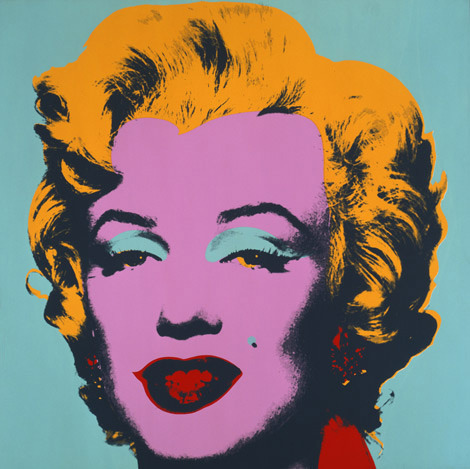
\includegraphics[width=0.68\textwidth]{art-marilyn}
    \caption{Popart slika umetnika Andyja Warhola~\cite{andyExhibitionMonroe}}
    \label{fig:art-marilyn}
\end{figure}

\section{Princip delovanja instalacije}
``15 sekund slave'' je interaktivna umetniška instalacija, ki obraz naključno
izbranega obiskovalca galerije povzdigne v umetniški objekt za petnajst
sekund~\cite{leonardo}. Instalacija je bila navdahnjena s slavnim citatom
Andyja Warhola: ``V prihodnosti bodo vsi ljudje doživeli svojih petnajst minut
slave.''\footnote{Originalno v angleščini: \textit{``In the future everybody
will be world-famous for fifteen minutes.''}\cite{andyExhibition,AW}.} pa tudi z
njegovim načinom predelave obrazov v slogu popart~\cite{solina200215}.



Če pogledamo sliko~\ref{fig:15sec}, vidimo le ``mojstrovino'', uokvirjeno v
dragocen okvir. V resnici pa se za to podobo skriva še mnogo več.

\begin{figure}
    \centering
    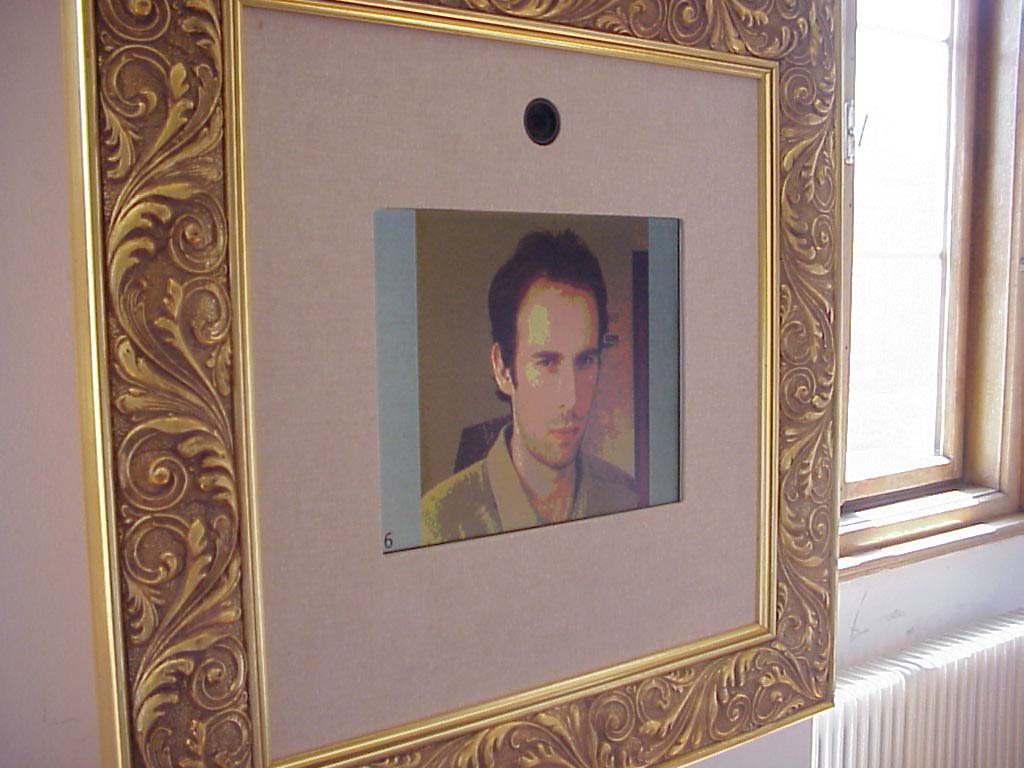
\includegraphics[width=0.7\textwidth]{15sec}
    \caption{Prikaz delovanja instalacije}
    \label{fig:15sec}
\end{figure}

Nad sliko obraza vidimo črno luknjo, to je prostor za digitalni fotoaparat, ki
enkrat na vsakih petnajst sekund fotografira okolico in fotografijo pošlje
računalniku, ki je skrit v ozadju. Fotoaparat ima širokokoten objektiv, da
lahko zajame čim širšo okolico.

Vsako novo fotografijo nato pošljemo računalniku, ki izvede algoritem za
iskanje obrazov. Če je teh več, enega izberemo po principu naključnega
izbora. Ta obraz izrežemo iz fotografije in ga pošljemo kot vhod
naslednjemu algoritmu.

Izbran obraz se obdela z enim izmed vnaprej določenih barvnih filtrov. Ti
filtri so sestavljeni iz različnih barvnih transformacij, da preoblikujejo
fotografijo v slogu popart.

Slika obraza v slogu popart je končni rezultat, ki je prikazan takoj, ko
prejšnjemu obrazu poteče njegovih petnajst sekund. In kako je prikazan? Pod
luknjo za fotoaparat je izrezan še večji pravokotnik, za katerim se skriva
računalniški zaslon LCD, povezan z računalnikom, ki je opravil
transformacijo fotografije.

Ta postopek se ponavlja v neskončnost, posebnost instalacije pa je, da se vse
dogaja v živo. Če bo torej nekdo dovolj dolgo gledal v okvir, ima veliko
možnosti, da bo kmalu zagledal samega sebe kot ``mojstrovino'' v
galeriji~\cite{lieser2010world}.


\chapter{Prvotna izvedba: 15 sekund slave}
\label{ch:prvotnaIzvedba15}
Kot že omenjeno, je prvotna instalacija nastala pred več kot desetimi leti. Ker
je težko nadomestiti le posamezne dele v sistemu in ker je tehnologija v teh
letih močno napredovala, se je pokazala potreba po prilagoditvi aplikacije
novemu stanju tehnologije~\cite{trifonova}.

\begin{figure}[!ht]
    \centering
    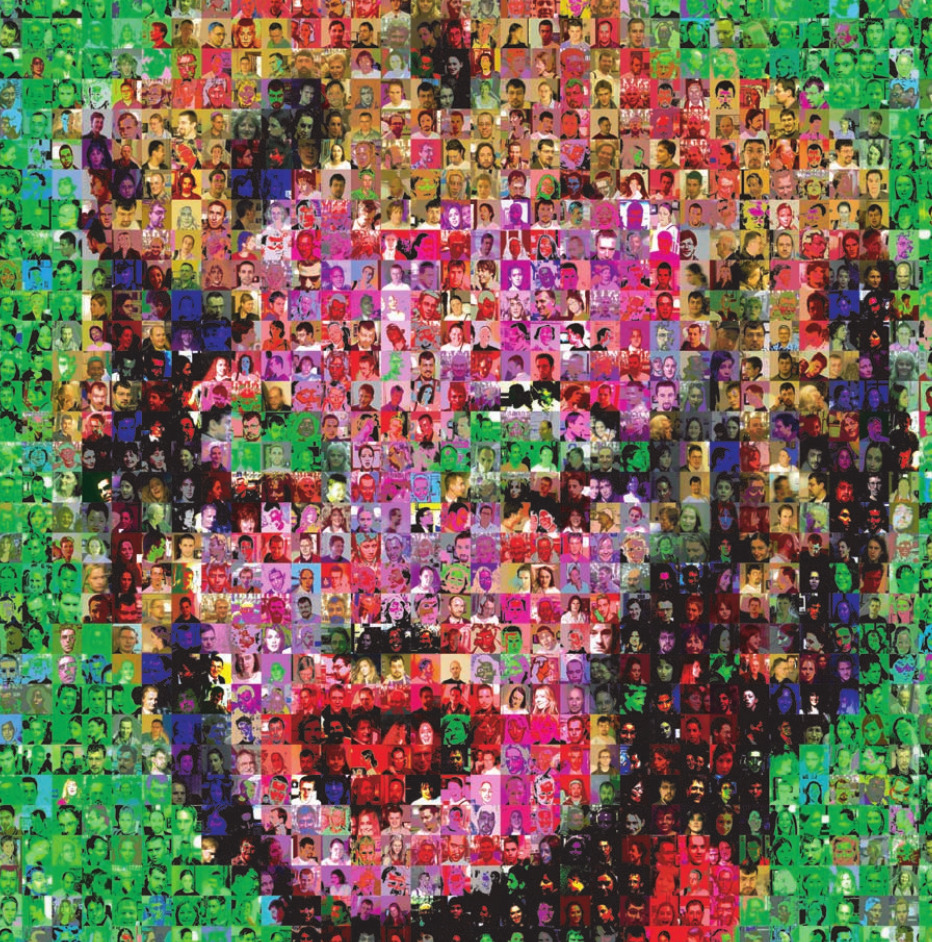
\includegraphics[width=0.68\textwidth]{15sec-marilyn}
    \caption{15 sekund slave slike umetnika Andyja Warhola~\cite{katalog_solina}}
    \label{fig:15sec-marilyn}
\end{figure}

\section{Strojna in programska oprema}
\paragraph{Strojna oprema.}
Prva razstavljena različica je imela bogato okrašen lesen okvir, ki pa ni bil
prenosen. Za tem okvirjem se je skrival računalniški zaslon LCD velikosti 17
palcev, malo nad tem zaslonom pa je bil fiksiran digitalni fotoaparat Olympus
C3020 ZOOM (objektiv tipa 32--96mm, maksimalna ločljivost je
2048$\times$1536)~\cite{preservationComputerBasedArt}.

Ob selitvi instalacije se je pripetila prva nadgradnja. Fiksen lesen okvir se
je zamenjal z razstavljivim in prenosljivim. V tem času je tudi tehnologija
naredila korak naprej. Naprave so postajale vse manjše in zmogljivejše. 17-palčni
računalniški zaslon je nadomestil 19-palčni, kljub temu pa se sama velikost
naprave ni povečala. Zamenjal se je tudi digitalni fotoaparat. Zaradi
programske opreme je bil najprimernejši kar Olympus, in ker je bil še vedno
željen široki kot objektiva, je to napravo nadomestil Olympus C40 ZOOM
(objektiv tipa 35--98mm, maksimalna ločljivost 2272$\times$1704).

Omenjeno je bilo, da je bil Olympus primeren zaradi programske opreme. Ta
digitalni fotoaparat je omogočal upravljanje same naprave programsko preko
računalnika. Orodje SDK omogoča nastavljanje ISO, odprtosti zaslonke, hitrosti
slikanja, fokusa, možnosti zajemanja slike ... S tem je omo\-go\-če\-no
avtomatsko zajemanje nove slike vsakih petnajst sekund.

\paragraph{Programska oprema.}
Modul za detekcijo obrazov je bil napisan v programskem jeziku C++. Sprva je
algoritem iskal obraze na podlagi barve kože. Zaradi hitrega in učinkovitega
delovanja je bila sama slika pomanjšana na resolucijo 160$\times$120 pikslov.
Najmanjši obraz, ki je bil lahko najden, je velikosti 11$\times$12 pikslov, največji
pa 96$\times$106 pikslov. Zaznavanje je bilo zelo občutljivo na svetlobo, še
posebej ob večjih spremembah med samim delovanjem. Za zmanjšanje tega problema
so se uporabljale različne metode za kompozicijo
osvetlitve~\cite{kovac2003illumination}. Kasneje se je celoten algoritem za
detekcijo obrazov zamenjal z algoritmom Viola-Jones~\cite{viola2004robust}, ki
pa ni bil več odvisen od barve kože. Najmanjši obraz pri algoritmu Viola-Jones
je bil velikosti 24$\times$24 pikslov.

Modul za filtre, s katerimi so se ustvarjali popart efekti, je bil prav tako
napisan v programskem jeziku C++. Slika obraza oziroma vhod, ki ga je
algoritem dobil, je bila slika velikosti 400$\times$400 pikslov. V kolikor je bil
rezultat detekcije obraza manjši, se je slika povečala na to velikost.

Komunikacija s samo strojno opremo in vsemi moduli je bila napisana v
programskem jeziku Pascal/Delphi. Celotna instalacija je bila narejena in
testirana na operacijskem sistemu Windows~XP~\cite{preservationComputerBasedArt}.


\chapter{Ohranjanje digitalne umetnosti}
\label{ch:ohranjanjeDigitalneUmetnosti}
Ohranjanje digitalne umetnosti je zelo pomembna vrednota v svetu
umetnosti~\cite{ZKM,preservationComputerBasedArt}. Navezuje se na umetnost, ki je sicer že v digitalni
obliki, a mora zaradi zelo hitrega razvoja tehnologije vseeno ostati v koraku
s časom. Novejša tehnologija nam omogoča zmogljivejše in hitrejše naprave, manjšo
porabo energije, bolj točne algoritme in še veliko drugih pomembnih izboljšav.
Vendar pa umetnost ni le tehnologija, umetnost je nekaj, kar naj bi se ohranjalo skozi
leta, desetletja, stoletja in še dlje.

Pri digitalni umetnosti se pojavi kar nekaj težav, ki jih pri ohranjanju
običajnih umetniških izdelkov ni. Če nismo v koraku s časom, je možnost, da
strojna oprema, ki jo potrebujemo za instalacijo, ni več dobavljiva na trgu
ali pa je že dovolj stara, da ima zgodovinsko vrednost. Nova strojna oprema
doprinese še programske posodobitve, nove principe, standarde in različna
delovanja. Zato je res pomembno, da sledimo razvoju, obenem pa se še vedno
trudimo, da zunanji obiskovalec kljub novi tehnologiji misli, da je to ista,
prvotna instalacija.

Četudi želimo zamenjati le strojno opremo, to v zelo starih instalacijah
ni mogoče. Stara programska oprema ne deluje vedno na novejših sistemih.
V tem primeru smo prisiljeni ponovno implementirati algoritme, tako da so
združljivi s strojno opremo. Tukaj obstaja več možnosti. Vedno lahko
uporabljamo staro kodo z manjšimi ali pa tudi večjimi popravki, tako da
se ta prevede tudi na novejših sistemih. Vendar pa je tu treba biti pozoren na
to, da si s tem ne povzročimo še več dela, kot če bi vse skupaj ponovno
implementirali.

Ko že govorimo o novi strojni in programski opremi, omenimo še drugo
težavo. Zaposleni v muzejih in galerijah običajno niso izobraženi za
vzdr\-že\-va\-nje digitalne umetnosti, saj ti ljudje načeloma niso strokovnjaki
računalniške stroke. Posledično so možne težave pri rokovanju s tako umetnino,
zato bi bilo priporočljivo, če bi bila instalacija podrobno dokumentirana in
bi bilo tako pojasnjeno, kako jo postaviti, kako jo vzdrževati in kaj storiti v
primeru težav.

Splošno gledano obstajata dve strategiji za ohranjanje digitalne umetnosti~\cite{ZKM}:
\begin{itemize}
\item
Ohraniti želimo vso strojno in programsko
opremo, dokler je to le mogoče. S tem zagotovimo, da je uporabniška izkušnja
ves čas enaka. Tukaj bi se večina lahko vprašala, zakaj ne bi strojne opreme s
časom nadgrajevali. Vzemimo za primer računalniški zaslon. Res je, tehnologija
LCD je zelo napredovala, slika je v primerjavi s sliko na zaslonih s katodno
cevjo precej bolj ostra in čista. Vendar pa ravno ta ostrina lahko
popolnoma spremeni končni produkt, saj je bil morda nekdo nad umetnino
navdušen ravno zaradi teh zabrisanih robov, ki so ji dajali nekoliko starinski
pridih.

\item
Nadgradimo strojno in programsko opremo. Pri tem
moramo biti zelo pazljivi, da uporabnik še vedno dobi tisto, kar je dobil pred
nadgradnjo. Umetniška instalacija mora ostati kar se da podobna prejšnji,
vključno z vsemi funkcionalnostmi. Vendar pa se pogosto zgodi, da avtor skozi
čas pridobi nove ideje za posodobitve, velikokrat gre tako za nekaj, kar prej
s staro tehnologijo sploh še ni bilo mogoče. Lep primer take ideje je
integracija s socialnimi omrežji.
\end{itemize}


\chapter{Nadgradnja: Naprava in pripomočki}
\label{ch:nadgradnjaNaprava}
Prvi motiv za nadgradnjo, ki smo si jo zamislili, je čim bolj učinkovito zmanjšati
porabljen prostor za instalacijo in s tem olajšati njeno prenosljivost in
povečati enostavnost postavitve.

Prvotna instalacija potrebuje osebni ali prenosni računalnik, zaslon LCD,
digitalni fotoaparat, mrežno opremo in dostop do interneta.

Kot najboljša zamenjava se je izkazala naprava `pametni telefon', saj ima
vse prej naštete naprave združene v eno. Ima vgrajeno kamero, ki služi kot
fotoaparat, dostop do interneta preko kartice SIM ter operacijski sistem, ki
omogoča izdelavo programske opreme, s katero lahko dostopamo do prej naštetih
funkcij.

Pametni telefoni višjega cenovnega razreda omogočajo tudi, da lahko sliko v živo
predvajamo na večjem ekranu. Zato smo se odločili, da kot testno napravo
vzamemo pametni telefon Samsung Galaxy S5.

\section{Testna naprava: Samsung Galaxy S5}
\label{sec:testnaNapravaSmartPhone}

\begin{figure}[!ht]
    \centering
    \begin{subfigure}[b]{0.4\textwidth}
        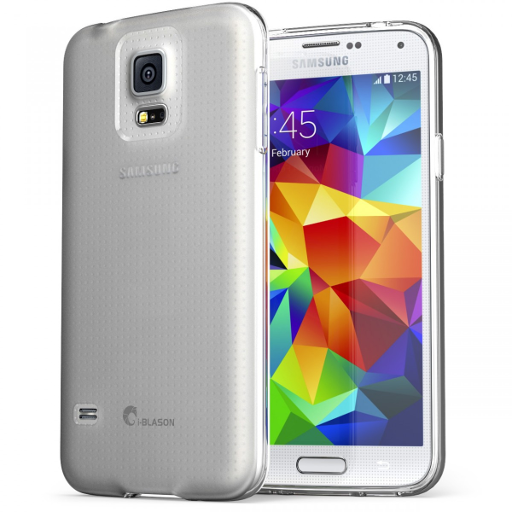
\includegraphics[width=\textwidth]{sgs5full}
    \end{subfigure}
    \begin{subfigure}[b]{0.4\textwidth}
        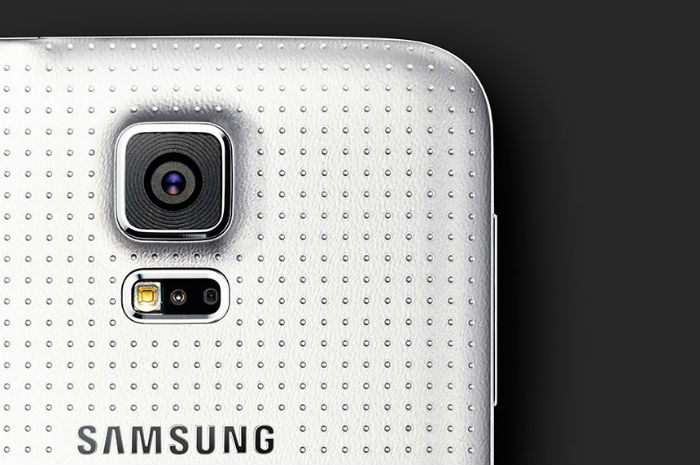
\includegraphics[width=\textwidth]{sgs5camera}
        \caption{Kamera z bliskavico}
    \end{subfigure}
    \caption{Testna naprava: Samsung Galaxy S5}
    \label{fig:sgs5}
\end{figure}

Samsung Galaxy S5 je pametni telefon, narejen v podjetju Samsung. Deluje z
operacijskim sistemom Android verzije 4.4.4, imenovanim tudi Android KitKat.
Trenutno najnovejša obstoječa verzija operacijskega sistema Android je 5.0,
poimenovan Lizika (\textit{angl. Lolipop}).

Samsung Galaxy S5 se ponaša s štirijedrnim procesorjem 2.5GHz Krait 400 na
čipu Qualcomm MSM8974AC Snapdragon 801. Ta procesor je dovolj zmogljiv za
preračunavanje vseh filtrov v zadovoljivem času.

Grafična enota, Adreno 330, omogoča prikazovanje v ločljivosti
1080$\times$1920 pikslov. Ena izmed pomembnih lastnosti je tudi možnost povezave
zunanje naprave preko priključka HDMI.

Tudi kamera je izjemno kvalitetna, je namreč tipa 1/2.6''. Svetlobno tipalo
ima 16 megapikslov in lahko torej naredi sliko v velikosti 5312$\times$2988
pikslov. Velikost in obliko kamere lahko vidimo kot majhen črn kvadrat, viden
na desni sliki~\ref{fig:sgs5}.

Pomembna lastnost je tudi operacijski sistem Android, za katerega je v
programskem jeziku Java mogoče napisati programsko opremo, imenovano
aplikacija. Vse, kar za to potrebujemo, je Android SDK in prevajalnik Java.


\section{Android}
\label{sec:android}
Android je odprtokodni sistem za pametne telefone, ki ga je leta 2007 izdelal
Open Handset Alliance pod vodstvom podjetja Google. Projekt se imenuje
AOSP~\footnote{Celotno ime je Android Open Source Project} in se še danes zelo
hitro razvija.

Temelji na jedru Linux, najbolj bistven del arhitekture pa je navidezni stroj
(\textit{angl. virtual machine}). Bolj podrobna zgradba sistema je prikazana
na sliki~\ref{picAndroid}. Navidezni stroj, imenovan Dalvik,
vsebuje prevajalnik JIT, ki je zadolžen za zaganjanje že prevedene programske
kode v javi. Prevedena koda je zapakirana v datoteke s končnico .apk. Tem
datotekam pravimo aplikacije, izdelane za sistem Android.

\begin{figure}
    \centering
    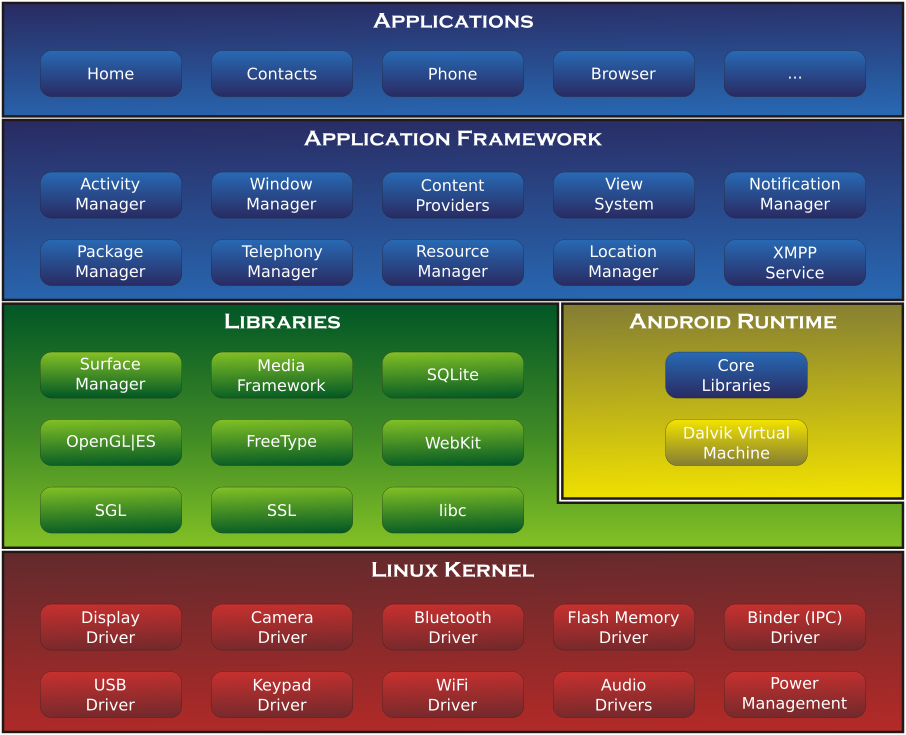
\includegraphics[width=\textwidth]{android}
    \caption{Struktura operacijskega sistema Android~\cite{wiki:Android}}
    \label{picAndroid}
\end{figure}

Za izdelavo aplikacije Android potrebujemo znanje programskega jezika Java,
Android SDK, ki je brezplačno na voljo na uradni spletni
strani\footnote{Uradna spletna stran je dostopna na {\tt
http://developer.android.com/}}. Priporočljivo je tudi branje dokumentacije
SDK, ki je na voljo na spletu\footnote{Dokumentacija SDK je dostopna na {\tt
http://developer.android.com/sdk/}}. Dokumentacija je napisana zelo
razumljivo, tako da se lahko znajdejo tudi začetniki. S pomočjo Android SDK na
koncu nastane datoteka .apk.


\chapter{Nadgradnja: Zaznavanje obrazov}
\label{ch:zaznavanjeObrazov}
Eden od pomembnih funkcionalnih elementov v instalaciji je avtomatska
detekcija  obrazov na slikah. V prvotni verziji instalacije je bila detekcija
obrazov izvedena s pomočjo barve kože~\cite{mirage03,kovac2003illumination}, od takrat pa je razvoj
na področju računalniškega vida prinesel veliko novosti in boljših metod.

Operacijski sistem Android nam preko vmesnika JNI omogoča vklju\-če\-va\-nje
kode, napisane v programskem jeziku C ali C++. Posledično lahko uporabljamo splošne knjižnice in
programska ogrodja (\textit{angl. framework}).

Ker smo v naši nadgradnji želeli, da bi se obrazi zaznavali v realnem času,
smo se odločili za uporabo programskega ogrodja OpenCV.


\section{Zaznavanje obrazov z uporabo OpenCV}
\label{sec:zaznavanjeObrazovOpenCV}
OpenCV je programsko ogrodje, ki nam omogoča izvedbo raznih operacij,
izvedenih nad slikami. Napisano je v programskem jeziku C, za potrebe
operacijskega sistema Android pa so napisani tudi povezovalni javanski razredi
(\textit{angl. class}), ki nam omogočajo uporabo operacij OpenCV kar v
programskem jeziku Java.

Najpomembnejša funkcionalnost programskega ogrodja OpenCV za nas je bila
implementacija zaznavanja obrazov. Ta uporablja algoritem kaskadnega
klasificiranja (\textit{angl. cascade classifier}), ki nam omogoča
klasifikacijo različnih lastnosti.

Lastnosti so zapisane v datoteki XML. Ta datoteka vsebuje več sto ali tisoč
različnih lastnosti, ki opisujejo določen predmet, v našem primeru obliko obraza.

Obstaja več različnih tipov, preko katerih so te lastnosti opisane. Za
zaznavanje obrazov sta najpomembnejša tipa HAAR in LBP. Tipa se
razlikujeta po točnosti in hitrosti.

Opisi HAAR so procesorsko bolj potratni in potrebujejo relativno veliko
časa za prepoznavo obraza, vendar pa je zato veliko manj napačnih detekcij
(\textit{angl. false positive}).

LBP pa je, čeprav z nekaj več napakami pri klasifikaciji kot HAAR, za
naše potrebe še vedno dovolj točen. Njegova glavna prednost pred prej
opisanim je njegova hitrost, kar je pri detekciji obrazov v živo zelo
pomembno, če želimo doseči zadovoljstvo uporabnika.

Ker so si obrazi med seboj zelo različni, je nemogoče, da bi bil najden prav
vsak obraz, vseeno pa želimo, da je število zgrešenih obrazov čim manjše.
Vendar pa zgrešen obraz ni največja težava, saj uporabnik tega najbrž ne bi
opazil. Veliko bolj neprijetna težava je, če najdemo obraz tam, kjer ga ni, na
primer nek predmet v okolici, ki ga zaznamo in obdelamo kot obraz.

Testirali smo oba tipa z različnimi tipi lastnosti. Pri tem smo uporabili le
lastnosti, ki opisujejo sprednji del obraza. Vendar pa se je pri uporabi
opisov LBP še vedno pokazalo preveč lažnih obrazov. Zato smo se odločili
za uporabo lastnosti tipa HAAR. Veliko bolj se nam namreč zdi pomembno, da
ima petnajst sekund slave obraz uporabnika, in ne kakšen predmet v okolici, pa
čeprav je za to potrebno nekoliko več časa.

Vendar pa tudi opisi obrazov tipa HAAR niso vedno dosegli našega
pri\-ča\-ko\-va\-nja. Zato smo se odločili, da naredimo dvojno klasifikacijo.

Najprej smo klasificirali z lastnostmi sprednjega dela obraza, opisanimi v
datoteki \textit{harrcascade\_frontalface\_default.xml}~\ref{lst:haar_frontal_face},
s katerimi smo dobili rezultate obrazov. Ker se je že za samo klasifikacijo
obraza porabilo kar nekaj časa, smo se odločili, da iskanje prekinemo takoj po
najdenem prvem obrazu, ki je velik vsaj eno desetino celotne slike.

\begin{lstlisting}[style=XML, label=lst:haar_frontal_face, caption=Nekaj vrstic datoteke harrcascade\_frontalface\_default.xml]
<maxWeakCount>9</maxWeakCount>
<stageThreshold>-5.0425500869750977e+00</stageThreshold>
<weakClassifiers>
  <_>
    <internalNodes>
      0 -1 0 -3.1511999666690826e-02
    </internalNodes>
    <leafValues>
      2.0875380039215088e+00 -2.2172100543975830e+00
    </leafValues>
  </_>
  <_>
    <internalNodes>
      0 -1 1 1.2396000325679779e-02
    </internalNodes>
    <leafValues>
      -1.8633940219879150e+00 1.3272049427032471e+00
    </leafValues>
  </_>
  ...
\end{lstlisting}

Kandidata obraza smo testirali še s klasifikacijo očesa. Vsak obraz ima dve
očesi. Zavedali smo se, da v primeru očal tega ne bomo našli, vendar pa se je
izkazalo, da težave nastopijo le pri zasenčenih očalih. Za to klasifikacijo smo
uporabili lastnosti, zapisane v datoteki \textit{harrcascade\_eye.xml}~\ref{lst:haar_eye}.
V primeru, da smo našli točno dva rezultata, smo vrnili prejšnji rezultat,
v nasprotnem primeru pa javili, da obraz ni najden.

\begin{lstlisting}[style=XML, label=lst:haar_eye, caption=Nekaj vrstic iz datoteke harrcascade\_eye.xml]
<maxWeakCount>6</maxWeakCount>
<stageThreshold>-1.4562760591506958e+00</stageThreshold>
<weakClassifiers>
  <_>
    <internalNodes>
      0 -1 0 1.2963959574699402e-01
    </internalNodes>
    <leafValues>
      -7.7304208278656006e-01 6.8350148200988770e-01
    </leafValues>
  </_>
  <_>
    <internalNodes>
      0 -1 1 -4.6326808631420135e-02
    </internalNodes>
    <leafValues>
      5.7352751493453979e-01 -4.9097689986228943e-01
    </leafValues>
  </_>
  ...
\end{lstlisting}

S temi nastavitvami in omejitvami smo dosegli pričakovane rezultate. Polje z
najdenim rezultatom smo povečali še za približno eno tretjino, tako da je
končni produkt zajemal nekoliko večji predel osnovne slike in je bil kvadratne
oblike. Zakaj ravno eno tretjino? Iskali smo prednji del obraza in ga tudi
našli. Vendar si v okvirju želimo videti sliko celotne glave in ne samo
obraza. Povečava polja za eno tretjino se je izkazala kot ravno pravšnja za
večino testiranih primerov.

\begin{figure}[!ht]
    \centering
    \begin{subfigure}[b]{0.3\textwidth}
        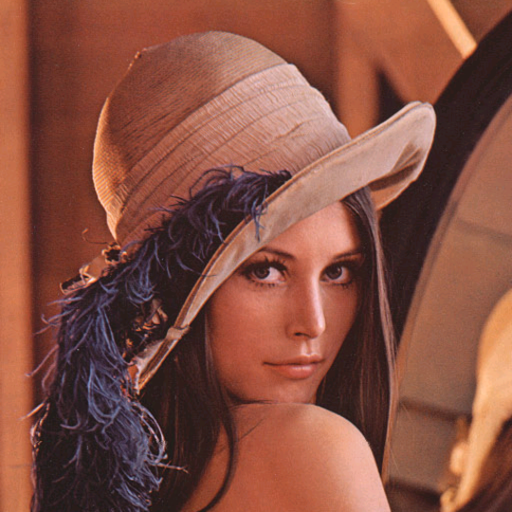
\includegraphics[width=\textwidth]{lena}
        \caption{Original}
    \end{subfigure}
    \begin{subfigure}[b]{0.3\textwidth}
        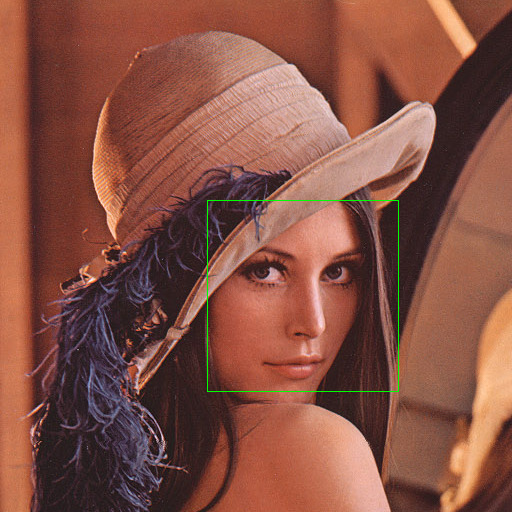
\includegraphics[width=\textwidth]{lena_opencv_face}
        \caption{Zaznavanje obraza}
        \label{fig:lena_opencv_face}
    \end{subfigure}
    \begin{subfigure}[b]{0.3\textwidth}
        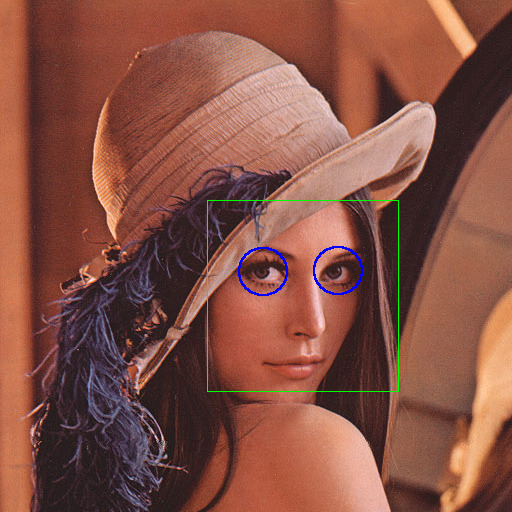
\includegraphics[width=\textwidth]{lena_opencv_face_eye}
        \caption{Zaznavanje oči}
        \label{fig:lena_opencv_face_eye}
    \end{subfigure}
    \caption{Prikaz zaznavanja obraza in oči s programskim ogrodjem OpenCV}
\end{figure}

Detekcija obrazov s programskim ogrodjem OpenCV je le ena izmed možnosti, ki
smo si jih podrobneje ogledali. Kot prva implementacija je bila izbrana zaradi
velike stopnje nadzora nad vsakim korakom, kot so: detekcija obraza,
prikazana kot zelen pravokotnik okrog obraza na
sliki~\ref{fig:lena_opencv_face}; določitev regije, kjer je potrebno iskati;
detekcija oči v določeni regiji, prikazana kot dva modra kroga okrog oči
na sliki~\ref{fig:lena_opencv_face_eye} in še bi lahko naštevali.

Kljub zadovoljivim rezultatom iskanja obrazov se je izkazalo, da slike
velikokrat niso ostre. Prej smo omenili, da imamo veliko nadzora nad
različnimi algoritmi za detekcijo, kar pa ne vključuje uporabe kamere, ki je v
pametnem telefonu. OpenCV uporablja sliko iz kamere tako, kot je, brez
predhodne izostritve. Povedano z drugimi besedami, uporablja jo kot kamero in
ne kot digitalni fotoaparat.


\section{Zaznavanje obrazov z uporabo Android SDK}
\label{sec:zaznavanjeObrazovAndroidSDK}
Android SDK deluje povsem drugače kot OpenCV. Ne omogoča nobenega nazdora in
parametrov, možna je uporaba le vnaprej določenega algoritma.

Ta algoritem temelji na algoritmu NV1-NORM~\cite{nevenFaceRecognition}, ki ga
je razvilo podjetje Neven Vision~\ref{fig:neven_vision}. Leta 2006 je Neven
Vision postalo last podjetja Google in od takrat se uporablja za zaznavo
obrazov v mnogih programih, ki jih je izdelalo podjetje Google. Lep  primer je
program za prikaz slik Google Picasa.

\begin{figure}[!ht]
    \centering
    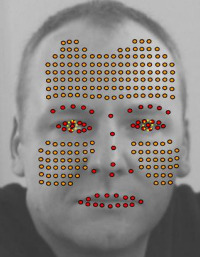
\includegraphics[width=0.3\textwidth]{neven_vision}
    \caption{Vizualizacija zaznavanja obraza, Neven Vision}
    \label{fig:neven_vision}
\end{figure}

Natančnejša implementacija algoritma za zaznavo obraza je zaprtokodna. Če si
ogledamo dokumentacijo Android SDK-ja, je opisan samo primer uporabe:
\begin{lstlisting}[style=java, caption=Primer uporabe zaznavanja obraza z orodjem Android SDK]
  FaceDetector fc = new FaceDetector(
      sirina_slike,
      visina_slike,
      maksimalno_stevilo_obrazov
  ).findFaces(slika, obrazi);
\end{lstlisting}

Vendar pa kljub zaprtosti in nezmožnosti prilagajanja detektorja prinaša zelo
dobre rezultate. Ker so vse funkcije že vključene v operacijski sistem, tudi
ne potrebujemo dodatnih programskih ogrodij. S tem smo si prihranili kar nekaj
časa in prostora.

Rezultat zaznavanja obraza pa tokrat ni obraz sam. Kot rezultat dobimo
razdaljo med očmi, rotacijo obraza ter točko med očmi. Na podlagi teh podatkov
lahko določimo regijo, na kateri je obraz na sliki.

Testirali smo razlike med rezultati obeh algoritmov in se na koncu odločili za
uporabo Android SDK. Kot že opisano, poleg dobrih rezultatov pridobimo še na
velikosti končne aplikacije in kompleksnosti celotnega programa.


\chapter{Nadgradnja: Obdelava slik}
\label{ch:obdelavaSlik}
Instalacija ``15 sekund slave'' vsebuje 17 različnih
filtrov~\cite[Poglavje~5]{thesisSamoJuvan} za predelavo slik obrazov v
popart portrete. Filtri so bili izdelani s pomočjo grafičnega programa GIMP.


\section{GIMP}
\label{sec:obdelavaSlikGIMP}
GIMP je odprtokodno programsko orodje za obdelavo slik.


Začetek projekta sega v leto 1995, kjer se je vse skupaj začelo kot
semestrski projekt na Univerzi Kalifornije, Berkeley. Avtorja Spencer Kimball
in Peter Mattis sta projekt poimenovala \textit{angl. General Image
Manipulation Program}, čez nekaj časa pa sta si premislila in Richarda
Stallmana, ki je ravno takrat obiskal univerzo, prosila, če lahko spremenita
``General'' v ``GNU''. Od takrat naprej se program imenuje
\textit{angl. GNU Image Manipulation Program} ali na kratko še vedno
GIMP~\cite{wiki:GIMP}.


\section{Izbira filtrov}
Že naša prvotna izbira filtrov je izhajala iz programskega orodja za predelavo
slik GIMP. Zaradi lažjega dela se je najprej s pomočjo grafičnega vmesnika
izbralo zaporedje različnih filtrov in njihove parametre. Izbrani so bili
naslednji filtri:
\begin{itemize}
    \item \textbf{uravnovešanje barv} \textit{angl. color balance} \hfill \\
        Prekrije celotno sliko z barvo v izbranem odtenku.
    \item \textbf{posteriziranje} \textit{angl. posterize} \hfill \\
        Zmanjšuje število barv na sliki.
    \item \textbf{uravnovešanje barv v prostoru HSL} \textit{angl. hue saturation balance} \hfill \\
        Spreminja odtenek, svetlost in nasičenost barv na sliki.
\end{itemize}

Iz teh treh filtrov je bilo narejenih mnogo kombinacij, v končni fazi pa
izbranih le 17 tistih, ki so bile najprimernejše. Ostale so bile izločene, ker
rezultati niso bili dovolj dobri, pri nekaterih pa je bila prevelika časovna
zahtevnost~\cite{thesisSamoJuvan}.


\section{Implementacija filtrov}
Ker je GIMP odprtokoden, smo imeli dostop tudi do implementacij filtrov.
Te so napisane v programskem jeziku C -- na prvi pogled kot
nalašč za enostaven prenos na platformo Android preko JNI. Vendar pa so se
pokazale težave, saj so bili filtri močno povezani z GIMP-objekti in nekoliko
bolj kompleksni, kot bi bilo potrebno za naš projekt. Zato smo se odločili, da
filtre ponovno implementiramo in zavržemo vse funkcionalnosti, ki za nas niso
pomembne. Naredili smo tri različne implementacije in jih med seboj primerjali.

Prva implementacija je napisana v programskem jeziku Java. Izkazala se je za
zelo počasno. Orodje za sproščanje pomnilnika GC \textit{(angl. garbage
collector)} se je klicalo prepogosto, kar je posledično porabilo več kot nekaj
sekund za filter. Tega si nismo mogli privoščiti, zato smo iskali alternative.

Naslednja implementacija je napisana s pomočjo grafične kartice, in sicer z
ogrodjem OpenGL ES verzije 2.0. Čas izvajanja se je občutno
zmanjšal. Ko so bile teksture zapisane na grafični kartici, so se filtri
izvajali v manj kot sekundi. Ta rešitev je bila že dovolj dobra, vendar pa se
nam je zdelo, da je uporaba grafične kartice za tako lahke operacije potrata
energije.

Čeprav so bili rezultati že dovolj dobri, smo se odločili še za implementacijo
v programskem jeziku C. Rezultati so pokazali, da je ta rešitev nekoliko
počasnejša kot prejšnja, vendar pa za to nismo potrebovali grafične kartice na
telefonu. Porabljen čas je bil manj kot sekundo za filter.


\subsection{Barvni prostor}
Ko govorimo o filtrih, govorimo predvsem o spreminjanju barv. Tukaj se pojavi
vprašanje: kako te barve matematično zapisati? Poznamo več barvnih
prostorov, s katerimi lahko določeni barvi priredimo določeno številko.


\subsubsection*{Barvni prostor RGB}
Najbolj znan in osnoven barvni prostor je RGB. Sestavljen je iz treh
osnovnih barv, to so rdeča (R), zelena (G) in modra (B). Vsaka barva se lahko
pojavi v 256 odtenkih, kar na koncu znaša $16777216$ barv ($256^3$).

\begin{figure}[!ht]
    \centering
    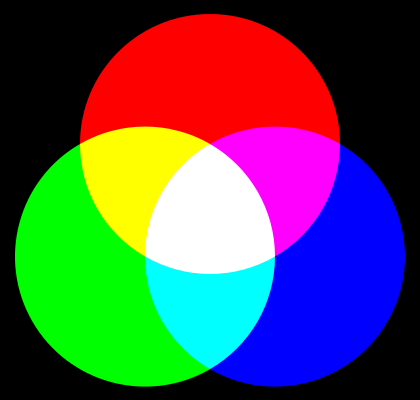
\includegraphics[width=0.4\textwidth]{rgb}
    \caption{Grafični prikaz barvnega prostora RGB}
    \label{fig:rgb}
\end{figure}


\subsubsection*{Barvni prostor HSL}
Drugi, malo manj znan, je barvni prostor HSL. Sestavljen je iz treh
komponent: barvni odtenek (H), intenzivnost (S) in svetlost (L). Če primerjamo
sliki~\ref{fig:rgb}~in~\ref{fig:hsl}, vidimo, da HSL nima treh enakih
komponent, ampak je zgrajen v obliki valja. Barvni odtenek je zapisan s
kotom, in sicer pri 0$^{\circ}$ se začne rdeča, pri 120$^{\circ}$ zelena in pri
240$^{\circ}$ modra. Drugi dve komponenti, nasičenost in svetlost, sta
zapisani z odstotki, in sicer od 0\% do 100\%.

\begin{figure}[!ht]
    \centering
    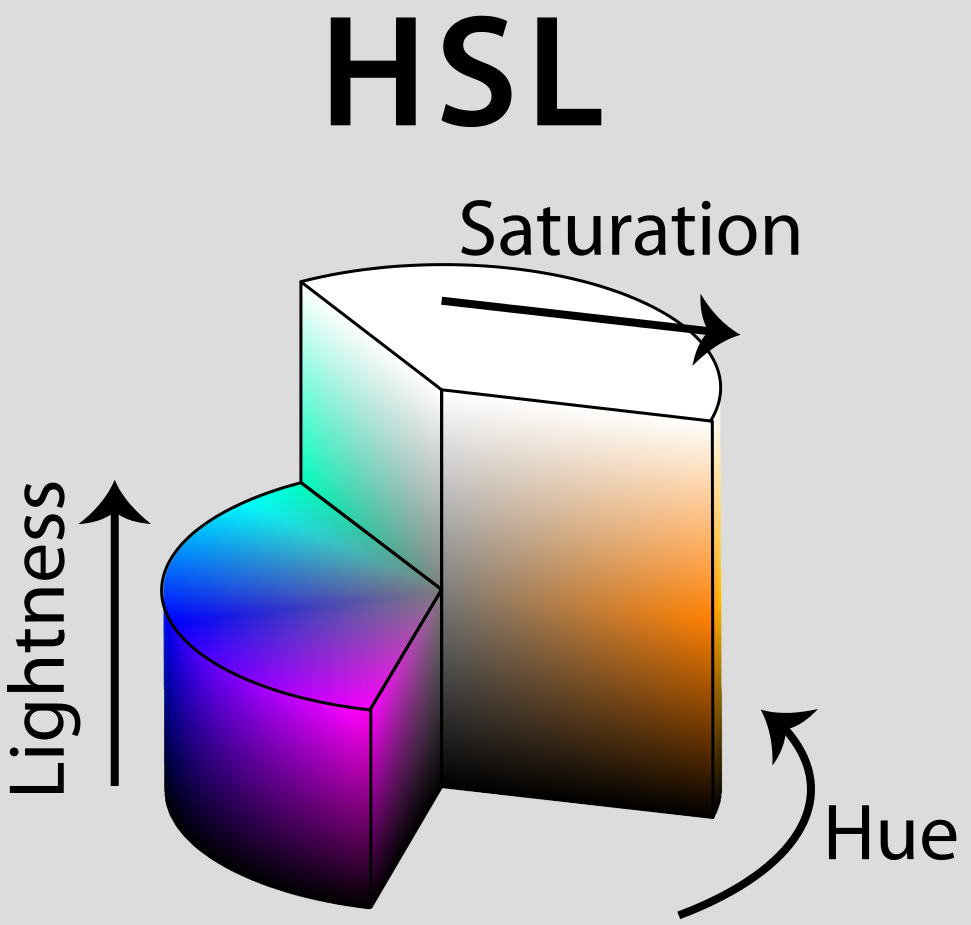
\includegraphics[width=0.4\textwidth]{hsl}
    \caption{Grafični prikaz barvnega prostora HSL}
    \label{fig:hsl}
\end{figure}

Obstaja še veliko barvnih prostorov, vendar sta za našo instalacijo
zadostovala ta dva. Pomembno pri barvnih modelih je tudi to, da so enostavno
preračunljivi iz enega prostora v drugega.


\subsection{Pretvorba iz barvnega modela RGB v HSL}
\label{sec:hslconvert}

\begin{align}
R, G, B &\in [0,255] \nonumber \\
Cmax &= max(R, G, B) \\
Cmin &= min(R, G, B) \\
\Delta &= (Cmax - Cmin)
\end{align}

\begin{equation}
L = (max + min) / 2 \label{eq:hsl_l}
\end{equation}

\begin{equation}
S =
\begin{cases}
    0 \text{,}& \Delta = 0 \\
    255 * \Delta / (Cmax + Cmin) \text{,}& L < 128 \\
    255 * \Delta / (511 - Cmax - Cmin) \text{,}& \text{ostalo}
\end{cases}
\end{equation}

\begin{equation}
H' =
\begin{cases}
    0 \text{,}& \Delta = 0 \\
    0 + 42.5 * (G - B) / \Delta \text{,}& R = Cmax \\
    85 + 42.5 * (B - R) / \Delta \text{,}& G = Cmax \\
    170 + 42.5 * (R - G) / \Delta \text{,}& B = Cmax
\end{cases}
\end{equation}

\begin{equation}
H =
\begin{cases}
    H' + 255 \text{,}& H' < 0 \\
    H' - 255 \text{,}& H' > 255 \\
    H' \text{,}& \text{ostalo}
\end{cases}
\end{equation}


\subsection{Uravnovešanje barv}
\label{sec:obdelavaSlikUravnovesanjeBarv}

\begin{equation}
clamp_{min}^{max}(x) =
\begin{cases}
    min \text{,}& x < min \\
    max \text{,}& x > max \\
    x \text{,}& \text{ostalo}
\end{cases}
\end{equation}

\begin{align}
shadows(x) &= clamp_{0}^{1}(\frac{117 - x}{64}) * 1.785 \\
color\_balance(x, x') &= clamp_{0}^{255}(x + x' * shadows(x)) \label{eq:color_balance}
\end{align}

Uravnovešanje barv se računa v barvnem prostoru RGB. Računamo za vsako
barvo posebej, in sicer z enačbo~\eqref{eq:color_balance}, kjer je $x$ enak
originalni barvi, $x'$ pa barvi, s katero želimo uravnovesiti originalno barvo
$x$. $x$ in $x'$ sta pozitivni celi števili med 0 in 255.

Po izračunanih vrednostih dane rezultate iz prostora RGB prenesemo v prostor HSL
s pomočjo enačb, napisanih v poglavju~\ref{sec:hslconvert}. Tako dobimo $H$,
$S$ in $L$. Iz originalne vrednosti, to je vrednost barve na sliki,
izračunamo $L$~\eqref{eq:hsl_l} in ga nadomestimo s prejšnjim, zato da ohranimo
podobno svetlost. $H$, $S$ in novo pridobljeni $L$ prenesemo nazaj v prostor RGB.


\subsection{Posteriziranje}
\label{sec:obdelavaSlikPosteriziranje}

\begin{equation}
luts(x, levels) = 255 * \frac{\left \lfloor{\frac{x}{255} * (levels - 1) + 0.5}\right \rfloor}{levels - 1} + 0.5 \label{eq:posterize}
\end{equation}

Posteriziranje se računa v barvnem prostoru RGB. Računamo za vsako barvo
posebej, in sicer z enačbo~\eqref{eq:posterize}, kjer je $x$ enak
originalni barvi, $levels$ pa je stopnja posteriziranja. $x$
in $levels$ sta pozitivni celi števili med 0 in 255.


\subsection{Uravnovešanje barv v prostoru HSL}
\label{sec:obdelavaSlikUravnovesanjeBarvHSL}

\begin{align}
htv(x, x') &= x + 255 * \frac{x'}{360} \nonumber \\
hue\_transfer(x, x') &=
\begin{cases}
    htv(x, x') + 255 \text{,}& htv(x, x') < 0 \\
    htv(x, x') - 255 \text{,}& htv(x, x') > 255 \\
    htv(x, x') \text{,}& \text{ostalo}
\end{cases} \label{eq:hue_transfer}
\end{align}

\begin{align}
ltv(x, x') &= clamp_{-255}^{255}(1.27 * x') \nonumber \\
lightness\_transfer(x, x') &=
\begin{cases}
    x * \frac{255 + ltv(x, x')}{255} \text{,}& ltv(x, x') < 0 \\
    x + \frac{(255 - x) * ltv(x, x')}{255} \text{,}& ltv(x, x') \geq 0
\end{cases} \label{eq:lightness_transfer}
\end{align}

\begin{align}
stv(x, x') &= clamp_{-255}^{255}(2.25 * x') \nonumber \\
saturation\_transfer(x, x') &= clamp_{0}^{255}(x + x * \frac{stv(x, x')}{255}) \label{eq:saturation_transfer}
\end{align}

Uravnovešanje barv v prostoru HSL se računa v barvnem prostoru HSL. Ker pa so
prvotno barve zapisane v barvnem prostoru RGB, je potrebno te pretvoriti v
barvni prostor HSL. To naredimo s pomočjo enačb, napisanih v
poglavju~\ref{sec:hslconvert}. Tako dobimo $H$, $S$ in $L$.

Zdaj lahko vsako komponento uravnovesimo. Vsaka komponenta se izra\-ču\-na po
svoji enačbi. Za $H$ uporabimo~\eqref{eq:hue_transfer}, za
$L$~\eqref{eq:lightness_transfer} in za $S$~\eqref{eq:saturation_transfer}.

Dobljene vrednosti pretvorimo nazaj v prostor RGB, kar je tudi naš rezultat.


\subsection{Sestavljanje popart filtrov}
\label{sec:obdelavaSlikSestavljanjePopArt}

\subsubsection*{Filter 1}
Prvi filter je sestavljen iz dveh osnovnih filtrov. Najprej sliko obdelamo s
filtrom ``uravnovešanje barv'', in sicer s parametri $R = 30$, $G = -32$ in
$B = 16$. Rezultat obdelamo še s filtrom ``posteriziranje'' s parametrom
$ST =4$. Rezultat testne slike lahko vidimo na sliki~\ref{fig:lena_filter_1}.

\begin{figure}[!ht]
    \centering
    \begin{subfigure}[b]{0.4\textwidth}
        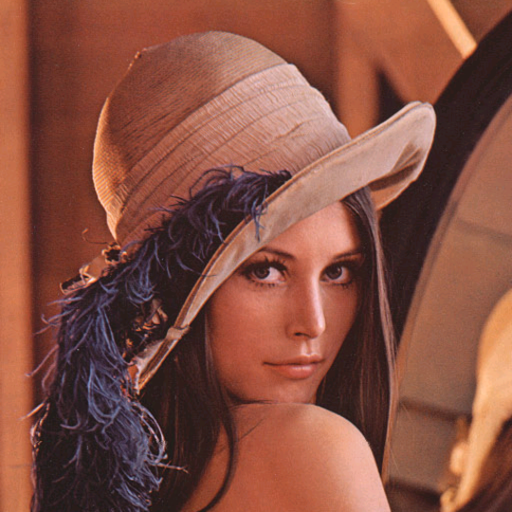
\includegraphics[width=\textwidth]{lena}
        \caption{Original}
    \end{subfigure}
    \begin{subfigure}[b]{0.4\textwidth}
        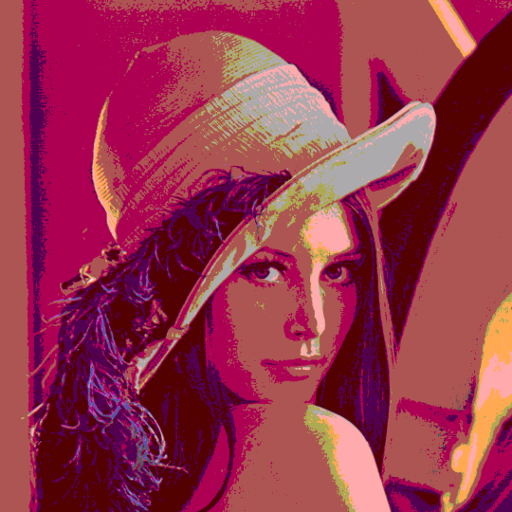
\includegraphics[width=\textwidth]{lena_filter_1}
        \caption{Prvi filter}
    \end{subfigure}
    \caption{Primerjava originalne slike s sliko, obdelano s filtrom št. 1}
    \label{fig:lena_filter_1}
\end{figure}


\subsubsection*{Filter 2}
Drugi filter je sestavljen iz dveh osnovnih filtrov. Najprej sliko obdelamo s
filtrom ``uravnovešanje barv'', in sicer s parametri $R = -36$, $G = -37$ in
$B = 39$. Rezultat obdelamo še s filtrom ``posteriziranje'' s parametrom
$ST = 4$. Rezultat testne slike lahko vidimo na sliki~\ref{fig:lena_filter_2}.

\begin{figure}[!ht]
    \centering
    \begin{subfigure}[b]{0.4\textwidth}
        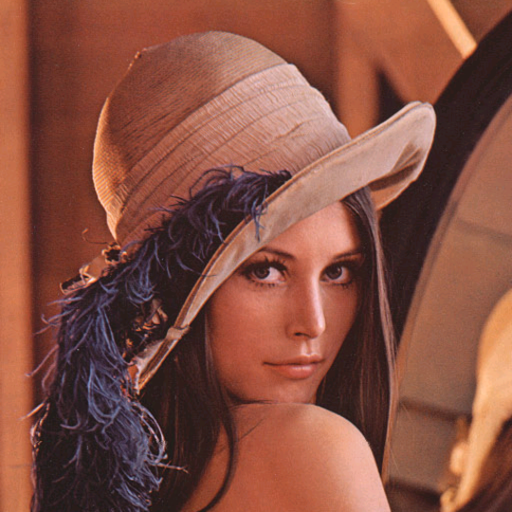
\includegraphics[width=\textwidth]{lena}
        \caption{Original}
    \end{subfigure}
    \begin{subfigure}[b]{0.4\textwidth}
        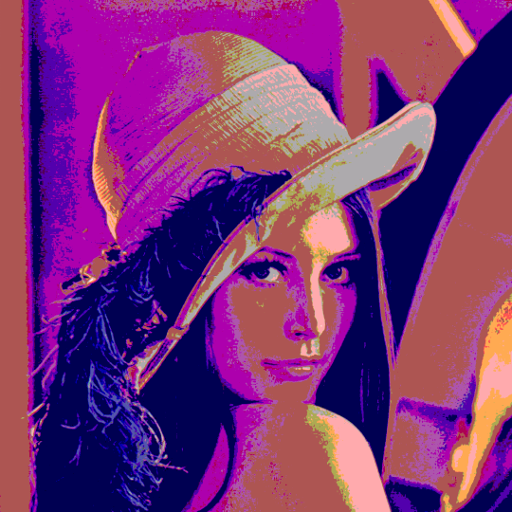
\includegraphics[width=\textwidth]{lena_filter_2}
        \caption{Drugi filter}
    \end{subfigure}
    \caption{Primerjava originalne slike s sliko, obdelano s filtrom št. 2}
    \label{fig:lena_filter_2}
\end{figure}


\subsubsection*{Filter 3}
Tretji filter vsebuje le osnovni filter ``posteriziranje'', in sicer s parametrom
$ST = 2$. Rezultat testne slike lahko vidimo na sliki~\ref{fig:lena_filter_3}.

\begin{figure}[!ht]
    \centering
    \begin{subfigure}[b]{0.4\textwidth}
        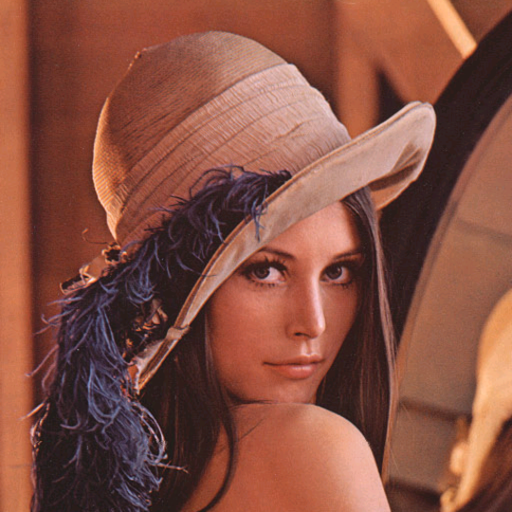
\includegraphics[width=\textwidth]{lena}
        \caption{Original}
    \end{subfigure}
    \begin{subfigure}[b]{0.4\textwidth}
        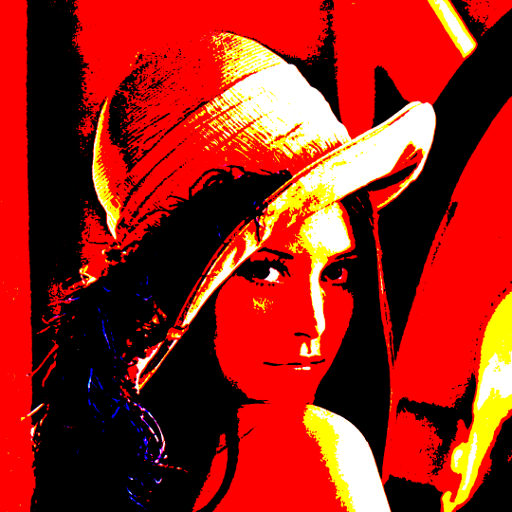
\includegraphics[width=\textwidth]{lena_filter_3}
        \caption{Tretji filter}
    \end{subfigure}
    \caption{Primerjava originalne slike s sliko, obdelano s filtrom št. 3}
    \label{fig:lena_filter_3}
\end{figure}


\subsubsection*{Filter 4}
Četrti filter je sestavljen iz dveh osnovnih filtrov. Najprej sliko obdelamo s
filtrom ``uravnovešanje barv'', in sicer s parametri $R = 100$, $G = -100$ in
$B = -100$. Rezultat obdelamo še s filtrom ``posteriziranje'' s parametrom
$ST = 3$. Rezultat testne slike lahko vidimo na sliki~\ref{fig:lena_filter_4}.

\begin{figure}[!ht]
    \centering
    \begin{subfigure}[b]{0.4\textwidth}
        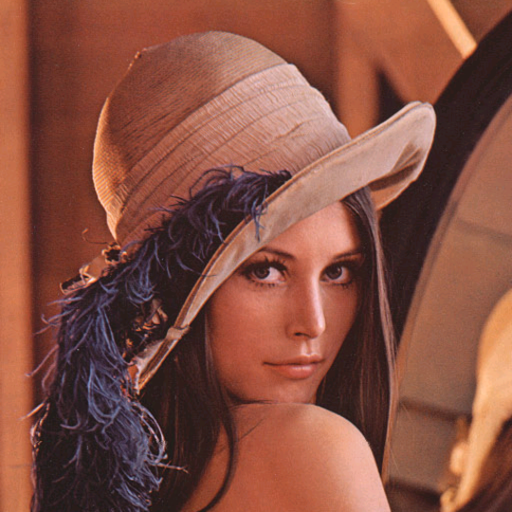
\includegraphics[width=\textwidth]{lena}
        \caption{Original}
    \end{subfigure}
    \begin{subfigure}[b]{0.4\textwidth}
        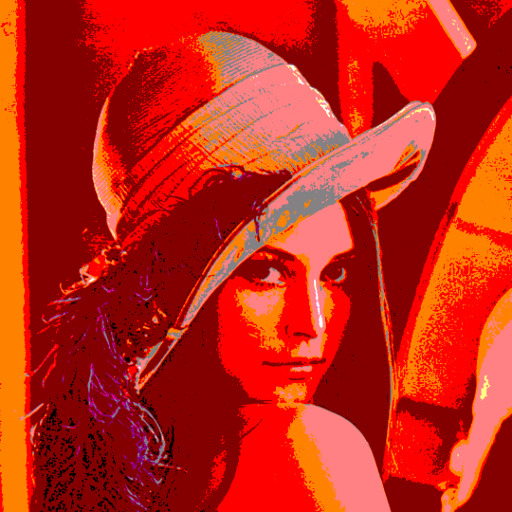
\includegraphics[width=\textwidth]{lena_filter_4}
        \caption{Četrti filter}
    \end{subfigure}
    \caption{Primerjava originalne slike s sliko, obdelano s filtrom št. 4}
    \label{fig:lena_filter_4}
\end{figure}


\subsubsection*{Filter 5}
Peti filter je sestavljen iz dveh osnovnih filtrov. Najprej sliko obdelamo s
filtrom ``uravnovešanje barv'', in sicer s parametri $R = -100$, $G = -100$ in
$B = 100$. Rezultat obdelamo še s filtrom ``posteriziranje'' s parametrom
$ST = 3$. Rezultat testne slike lahko vidimo na sliki~\ref{fig:lena_filter_5}.

\begin{figure}[!ht]
    \centering
    \begin{subfigure}[b]{0.4\textwidth}
        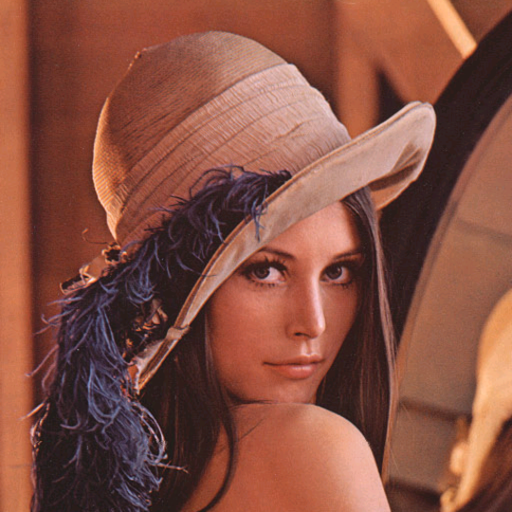
\includegraphics[width=\textwidth]{lena}
        \caption{Original}
    \end{subfigure}
    \begin{subfigure}[b]{0.4\textwidth}
        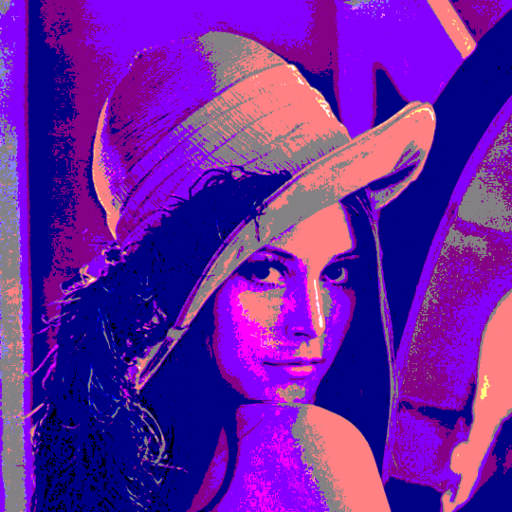
\includegraphics[width=\textwidth]{lena_filter_5}
        \caption{Peti filter}
    \end{subfigure}
    \caption{Primerjava originalne slike s sliko, obdelano s filtrom št. 5}
    \label{fig:lena_filter_5}
\end{figure}


\subsubsection*{Filter 6}
Šesti filter je sestavljen iz dveh osnovnih filtrov. Najprej sliko obdelamo s
filtrom ``uravnovešanje barv'', in sicer s parametri $R = -100$, $G = 100$ in
$B = -100$. Rezultat obdelamo še s filtrom ``posteriziranje'' s parametrom
$ST = 3$. Rezultat testne slike lahko vidimo na sliki~\ref{fig:lena_filter_6}.

\begin{figure}[!ht]
    \centering
    \begin{subfigure}[b]{0.4\textwidth}
        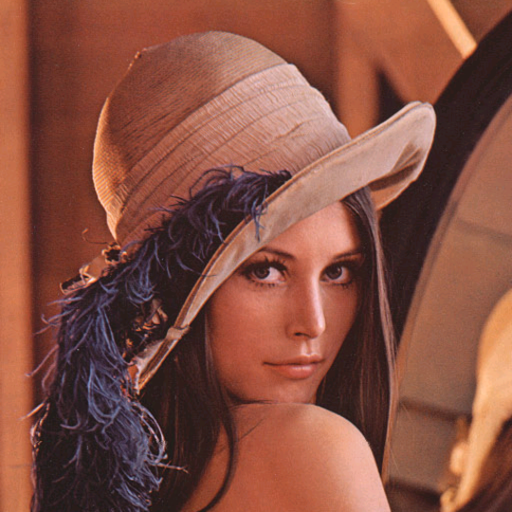
\includegraphics[width=\textwidth]{lena}
        \caption{Original}
    \end{subfigure}
    \begin{subfigure}[b]{0.4\textwidth}
        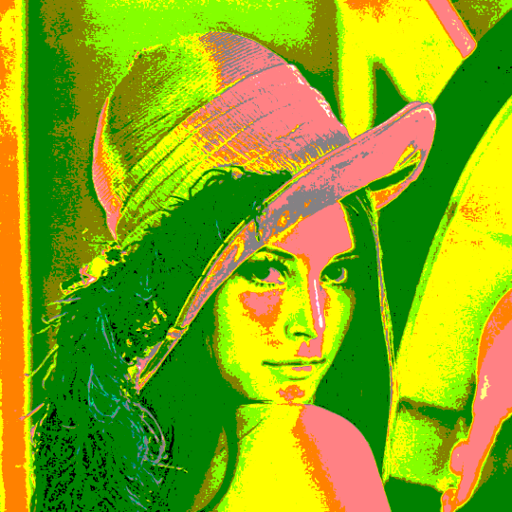
\includegraphics[width=\textwidth]{lena_filter_6}
        \caption{Šesti filter}
    \end{subfigure}
    \caption{Primerjava originalne slike s sliko, obdelano s filtrom št. 6}
    \label{fig:lena_filter_6}
\end{figure}


\subsubsection*{Filter 7}
Sedmi filter je sestavljen iz dveh osnovnih filtrov. Najprej sliko obdelamo s
filtrom ``posteriziranje'', in sicer s parametrom $ST = 5$. Rezultat obdelamo
še s filtrom ``uravnovešanje barv v prostoru HSL'' s parametri $H = -41$,
$L = -15$ in $S = 6$. Rezultat testne slike lahko vidimo na
sliki~\ref{fig:lena_filter_7}.

\begin{figure}[!ht]
    \centering
    \begin{subfigure}[b]{0.4\textwidth}
        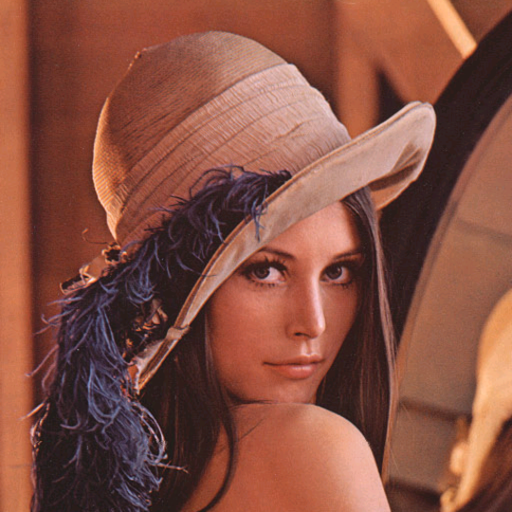
\includegraphics[width=\textwidth]{lena}
        \caption{Original}
    \end{subfigure}
    \begin{subfigure}[b]{0.4\textwidth}
        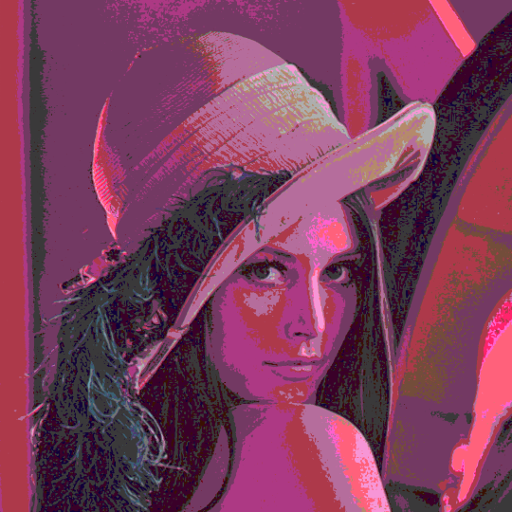
\includegraphics[width=\textwidth]{lena_filter_7}
        \caption{Sedmi filter}
    \end{subfigure}
    \caption{Primerjava originalne slike s sliko, obdelano s filtrom št. 7}
    \label{fig:lena_filter_7}
\end{figure}


\subsubsection*{Filter 8}
Osmi filter je sestavljen iz dveh osnovnih filtrov. Najprej sliko obdelamo s
filtrom ``posteriziranje'', in sicer s parametrom $ST = 6$. Rezultat obdelamo
še s filtrom ``uravnovešanje barv'' s parametri $R = -29$, $G = 40$ in $B = 100$.
Rezultat testne slike lahko vidimo na sliki~\ref{fig:lena_filter_8}.

\begin{figure}[!ht]
    \centering
    \begin{subfigure}[b]{0.4\textwidth}
        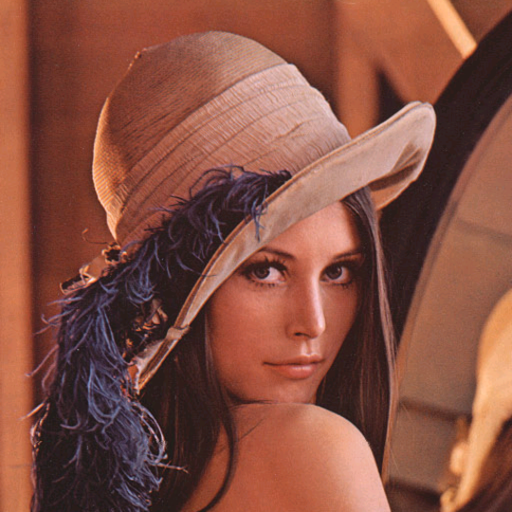
\includegraphics[width=\textwidth]{lena}
        \caption{Original}
    \end{subfigure}
    \begin{subfigure}[b]{0.4\textwidth}
        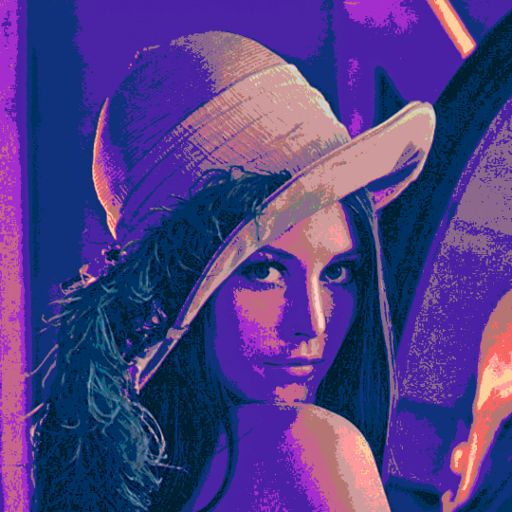
\includegraphics[width=\textwidth]{lena_filter_8}
        \caption{Osmi filter}
    \end{subfigure}
    \caption{Primerjava originalne slike s sliko, obdelano s filtrom št. 8}
    \label{fig:lena_filter_8}
\end{figure}


\subsubsection*{Filter 9}
Deveti filter je sestavljen iz dveh osnovnih filtrov. Najprej sliko obdelamo s
filtrom ``uravnovešanje barv v prostoru HSL'', in sicer s parametri $H = -41$,
$L = -20$ in $S = 25$. Rezultat obdelamo še s filtrom ``posteriziranje'' s
parametrom $ST = 4$. Rezultat testne slike lahko vidimo na
sliki~\ref{fig:lena_filter_9}.

\begin{figure}[!ht]
    \centering
    \begin{subfigure}[b]{0.4\textwidth}
        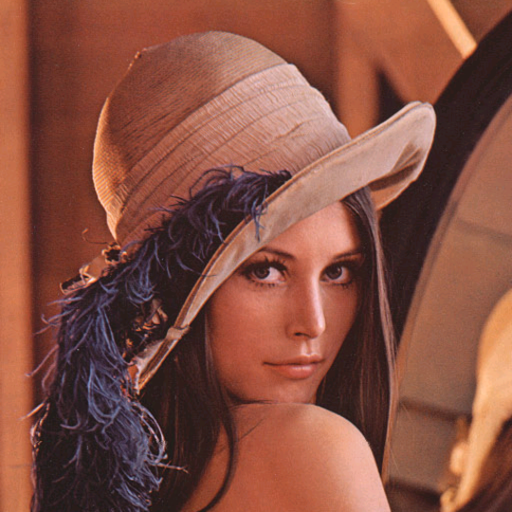
\includegraphics[width=\textwidth]{lena}
        \caption{Original}
    \end{subfigure}
    \begin{subfigure}[b]{0.4\textwidth}
        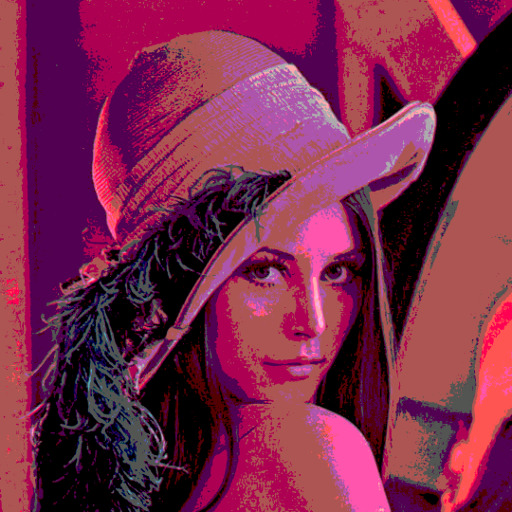
\includegraphics[width=\textwidth]{lena_filter_9}
        \caption{Deveti filter}
    \end{subfigure}
    \caption{Primerjava originalne slike s sliko, obdelano s filtrom št. 9}
    \label{fig:lena_filter_9}
\end{figure}


\subsubsection*{Filter 10}
Deseti filter je sestavljen iz treh osnovnih filtrov. Najprej sliko obdelamo s
filtrom ``uravnovešanje barv'', in sicer s parametri $R = 100$, $G = -100$ in
$B = -100$. Rezultat obdelamo še s filtrom ``posteriziranje'' s parametrom
$ST= 3$ in nazadnje še s filtrom ``uravnovešanje barv v prostoru HSL'' s
parametri $H = -41$, $L = -10$ in $S = 20$. Rezultat testne slike lahko
vidimo na sliki~\ref{fig:lena_filter_10}.

\begin{figure}[!ht]
    \centering
    \begin{subfigure}[b]{0.4\textwidth}
        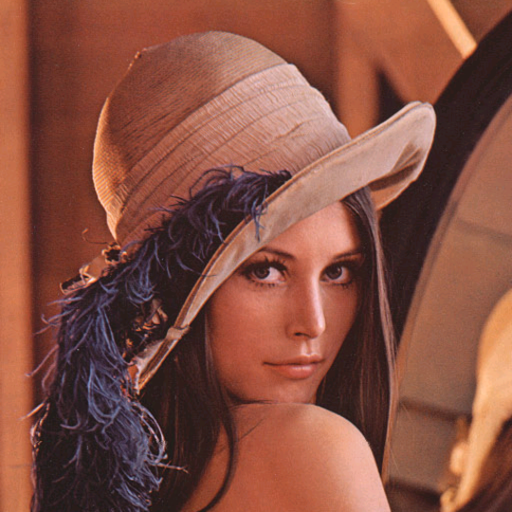
\includegraphics[width=\textwidth]{lena}
        \caption{Original}
    \end{subfigure}
    \begin{subfigure}[b]{0.4\textwidth}
        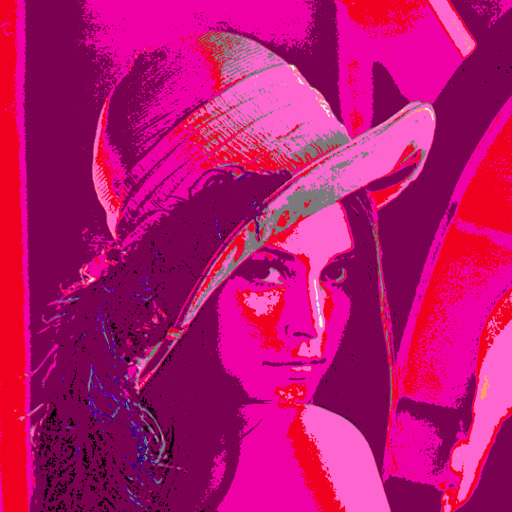
\includegraphics[width=\textwidth]{lena_filter_10}
        \caption{Deseti filter}
    \end{subfigure}
    \caption{Primerjava originalne slike s sliko, obdelano s filtrom št. 10}
    \label{fig:lena_filter_10}
\end{figure}


\subsubsection*{Filter 11}
Enajsti filter je sestavljen iz treh osnovnih filtrov. Najprej sliko obdelamo s
filtrom ``uravnovešanje barv'', in sicer s parametri $R = 34$, $G = -38$ in
$B = 24$. Rezultat obdelamo še s filtrom ``posteriziranje'' s parametrom
$ST= 4$ in nazadnje še s filtrom ``uravnovešanje barv v prostoru HSL'' s
parametri $H = -65$, $L = 0$ in $S = 0$. Rezultat testne slike lahko
vidimo na sliki~\ref{fig:lena_filter_11}.

\begin{figure}[!ht]
    \centering
    \begin{subfigure}[b]{0.4\textwidth}
        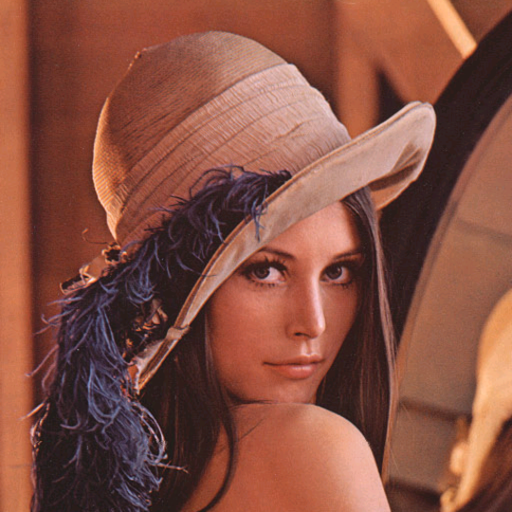
\includegraphics[width=\textwidth]{lena}
        \caption{Original}
    \end{subfigure}
    \begin{subfigure}[b]{0.4\textwidth}
        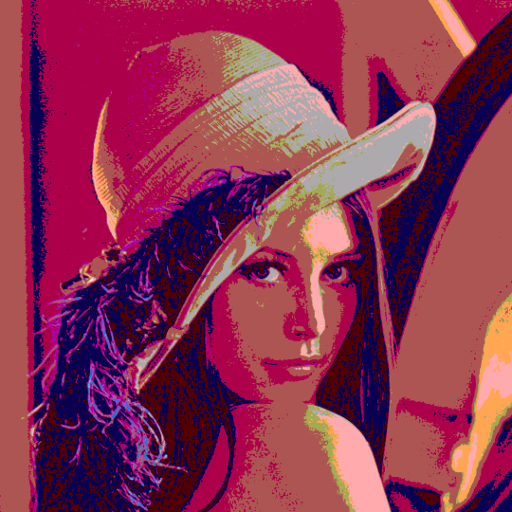
\includegraphics[width=\textwidth]{lena_filter_11}
        \caption{Enajsti filter}
    \end{subfigure}
    \caption{Primerjava originalne slike s sliko, obdelano s filtrom št. 11}
    \label{fig:lena_filter_11}
\end{figure}


\subsubsection*{Filter 12}
Dvanajsti filter je sestavljen iz dveh osnovnih filtrov. Najprej sliko obdelamo s
filtrom ``uravnovešanje barv'', in sicer s parametri $R = 40$, $G = -40$ in
$B = 28$. Rezultat obdelamo še s filtrom ``posteriziranje'' s parametrom
$ST= 4$ in nazadnje še enkrat s filtrom ``uravnovešanje barv'', vendar s
parametri $R = -100$, $G = -42$ in $B = 100$. Rezultat testne slike lahko
vidimo na sliki~\ref{fig:lena_filter_12}.

\begin{figure}[!ht]
    \centering
    \begin{subfigure}[b]{0.4\textwidth}
        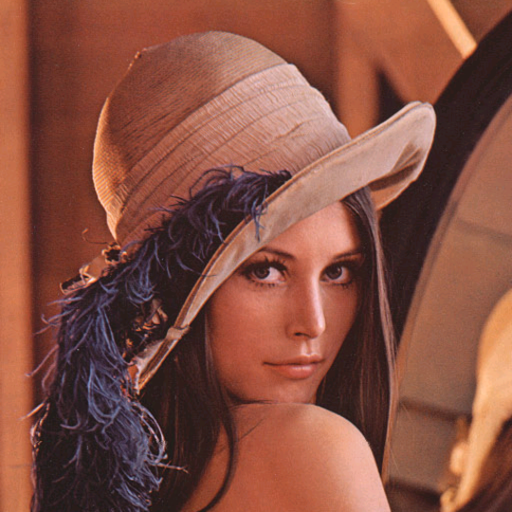
\includegraphics[width=\textwidth]{lena}
        \caption{Original}
    \end{subfigure}
    \begin{subfigure}[b]{0.4\textwidth}
        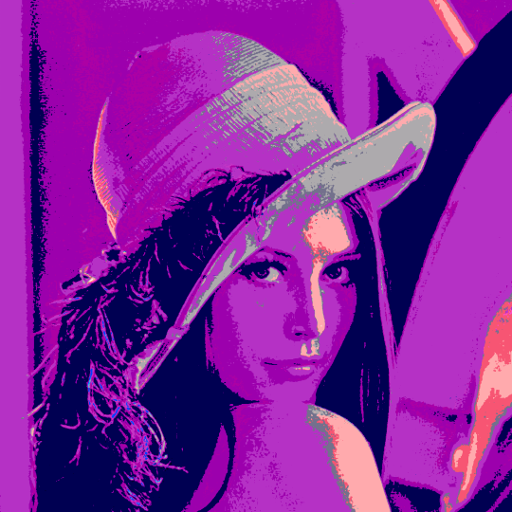
\includegraphics[width=\textwidth]{lena_filter_12}
        \caption{Dvanajsti filter}
    \end{subfigure}
    \caption{Primerjava originalne slike s sliko, obdelano s filtrom št. 12}
    \label{fig:lena_filter_12}
\end{figure}


\subsubsection*{Filter 13}
Trinajsti filter je sestavljen iz dveh osnovnih filtrov. Najprej sliko obdelamo s
filtrom ``uravnovešanje barv'', in sicer s parametri $R = 45$, $G = -45$ in
$B = 35$. Rezultat obdelamo še s filtrom ``posteriziranje'' s parametrom
$ST =4$. Rezultat testne slike lahko vidimo na sliki~\ref{fig:lena_filter_13}.

\begin{figure}[!ht]
    \centering
    \begin{subfigure}[b]{0.4\textwidth}
        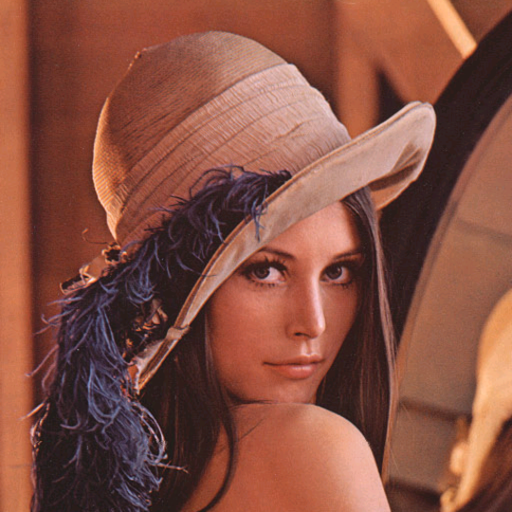
\includegraphics[width=\textwidth]{lena}
        \caption{Original}
    \end{subfigure}
    \begin{subfigure}[b]{0.4\textwidth}
        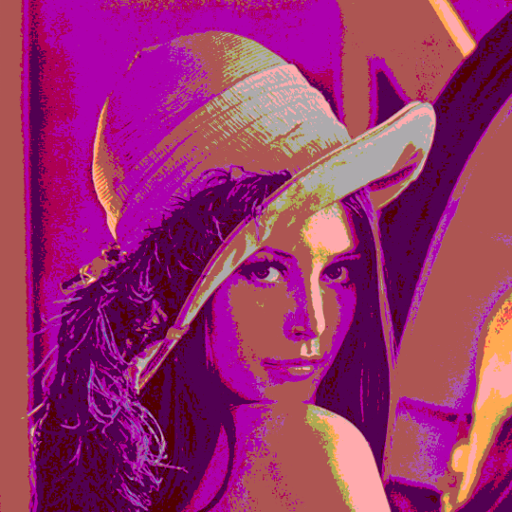
\includegraphics[width=\textwidth]{lena_filter_13}
        \caption{Trinajsti filter}
    \end{subfigure}
    \caption{Primerjava originalne slike s sliko, obdelano s filtrom št. 13}
    \label{fig:lena_filter_13}
\end{figure}


\subsubsection*{Filter 14}
Štirinajsti filter je sestavljen iz dveh osnovnih filtrov. Najprej sliko obdelamo s
filtrom ``uravnovešanje barv'', in sicer s parametri $R = -45$, $G = -55$ in
$B = 30$. Rezultat obdelamo še s filtrom ``posteriziranje'' s parametrom
$ST =4$. Rezultat testne slike lahko vidimo na sliki~\ref{fig:lena_filter_14}.

\begin{figure}[!ht]
    \centering
    \begin{subfigure}[b]{0.4\textwidth}
        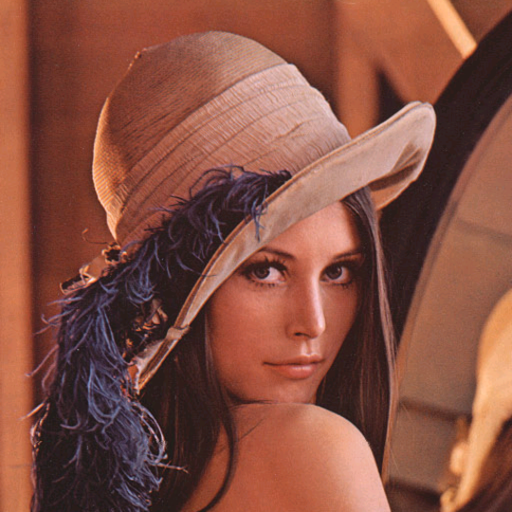
\includegraphics[width=\textwidth]{lena}
        \caption{Original}
    \end{subfigure}
    \begin{subfigure}[b]{0.4\textwidth}
        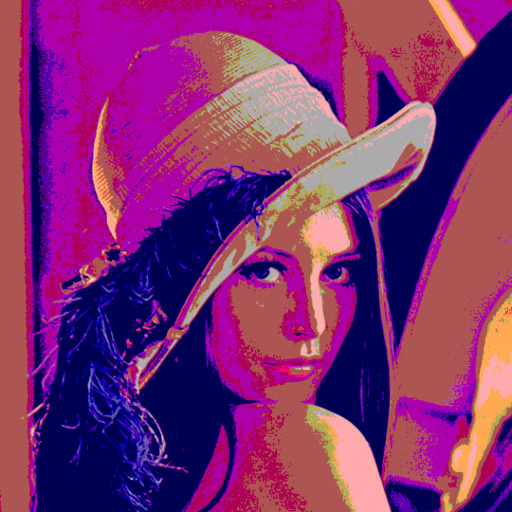
\includegraphics[width=\textwidth]{lena_filter_14}
        \caption{Štirinajsti filter}
    \end{subfigure}
    \caption{Primerjava originalne slike s sliko, obdelano s filtrom št. 14}
    \label{fig:lena_filter_14}
\end{figure}


\subsubsection*{Filter 15}
Petnajsti filter vsebuje le osnovni filter ``posteriziranje'', in sicer s parametrom
$ST = 3$. Rezultat testne slike lahko vidimo na sliki~\ref{fig:lena_filter_15}.

\begin{figure}[!ht]
    \centering
    \begin{subfigure}[b]{0.4\textwidth}
        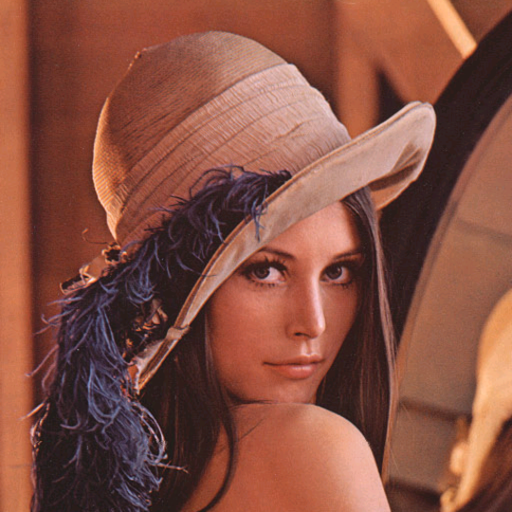
\includegraphics[width=\textwidth]{lena}
        \caption{Original}
    \end{subfigure}
    \begin{subfigure}[b]{0.4\textwidth}
        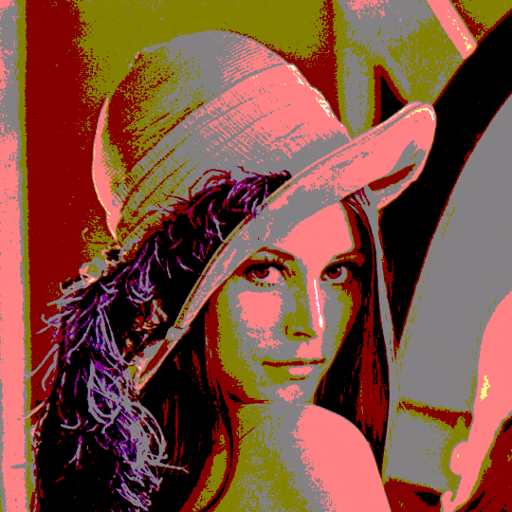
\includegraphics[width=\textwidth]{lena_filter_15}
        \caption{Petnajsti filter}
    \end{subfigure}
    \caption{Primerjava originalne slike s sliko, obdelano s filtrom št. 15}
    \label{fig:lena_filter_15}
\end{figure}


\subsubsection*{Filter 16}
Šestnajsti filter je sestavljen iz dveh osnovnih filtrov. Najprej sliko obdelamo s
filtrom ``uravnovešanje barv'', in sicer s parametri $R = 30$, $G = -40$ in
$B = 16$. Rezultat obdelamo še s filtrom ``posteriziranje'' s parametrom
$ST =3$. Rezultat testne slike lahko vidimo na sliki~\ref{fig:lena_filter_16}.

\begin{figure}[!ht]
    \centering
    \begin{subfigure}[b]{0.4\textwidth}
        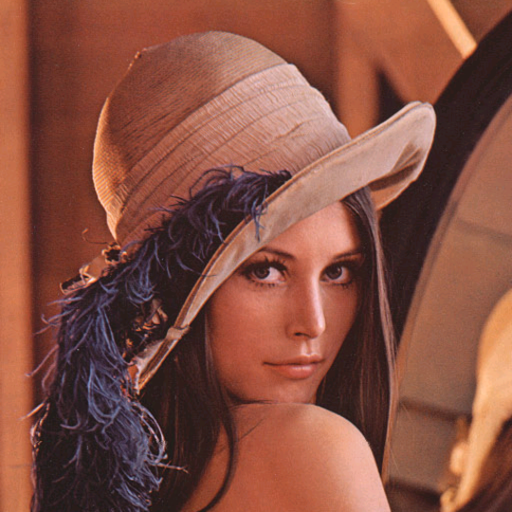
\includegraphics[width=\textwidth]{lena}
        \caption{Original}
    \end{subfigure}
    \begin{subfigure}[b]{0.4\textwidth}
        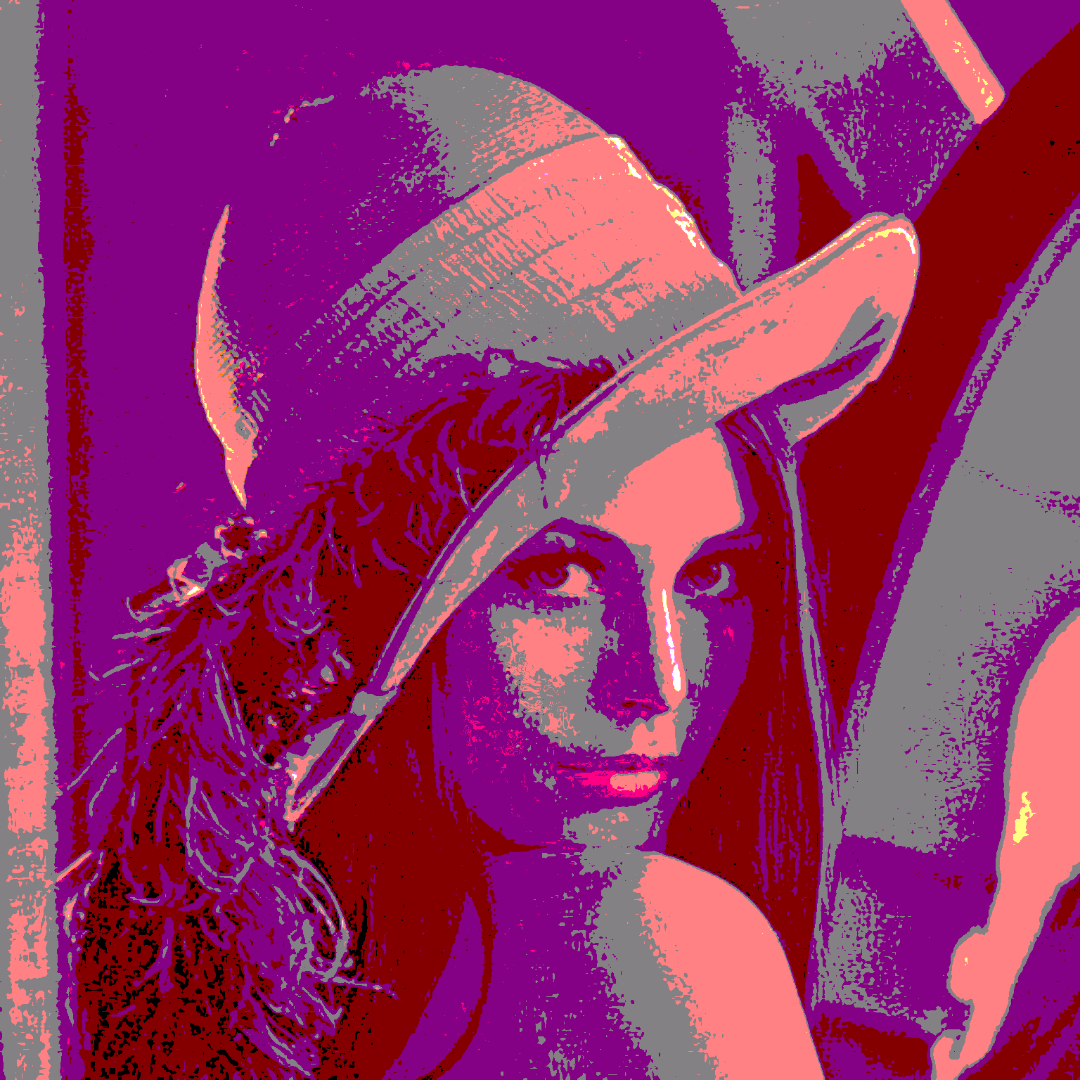
\includegraphics[width=\textwidth]{lena_filter_16}
        \caption{Šestnajsti filter}
    \end{subfigure}
    \caption{Primerjava originalne slike s sliko, obdelano s filtrom št. 16}
    \label{fig:lena_filter_16}
\end{figure}


\subsubsection*{Filter 17}
Sedemnajsti filter je sestavljen iz treh osnovnih filtrov. Najprej sliko obdelamo s
filtrom ``uravnovešanje barv'', in sicer s parametri $R = 20$, $G = -30$ in
$B = 20$. Rezultat obdelamo še s filtrom ``posteriziranje'' s parametrom
$ST= 4$ in nazadnje še s filtrom ``uravnovešanje barv v prostoru HSL'' s
parametri $H = -30$, $L = -10$ in $S = 12$. Rezultat testne slike lahko
vidimo na sliki~\ref{fig:lena_filter_17}.

\begin{figure}[!ht]
    \centering
    \begin{subfigure}[b]{0.4\textwidth}
        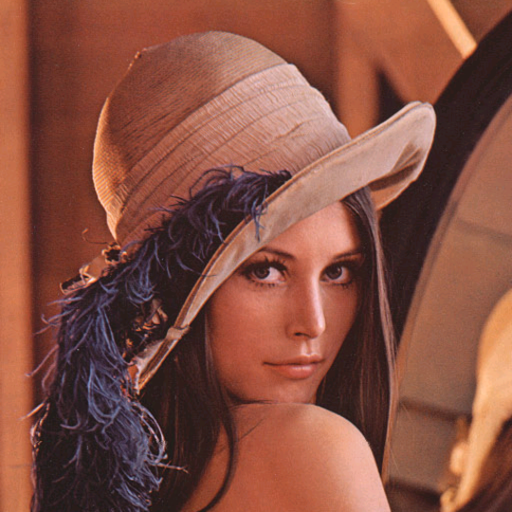
\includegraphics[width=\textwidth]{lena}
        \caption{Original}
    \end{subfigure}
    \begin{subfigure}[b]{0.4\textwidth}
        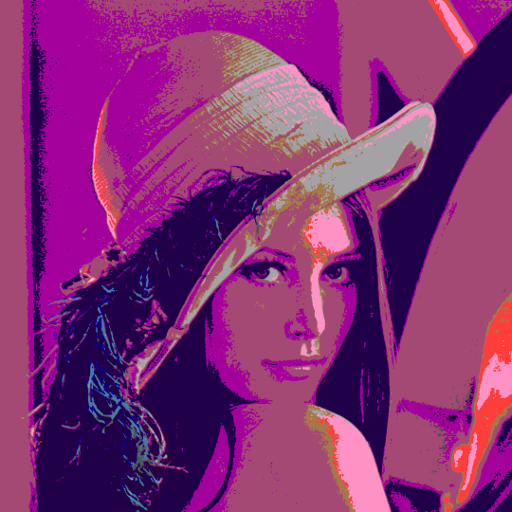
\includegraphics[width=\textwidth]{lena_filter_17}
        \caption{Sedemnajsti filter}
    \end{subfigure}
    \caption{Primerjava originalne slike s sliko, obdelano s filtrom št. 17}
    \label{fig:lena_filter_17}
\end{figure}


\chapter{Nove funkcionalne možnosti}
\label{ch:novosti}
Do sedaj smo originalno instalacijo ``15 sekund slave'' predelovali na način,
da jo ohranjamo kot digitalno umetnost, se pravi brez vidnih sprememb. Vendar
pa kakšna manjša po tako dolgem času lahko uporabniško izkušnjo le popestri.

Najpomembnejša posodobitev, ki bi to umetniško instalacijo naredila veliko
bolj popularno, je integracija s socialnimi omrežji, kar je podrobneje opisano
v~\ref{ch:socialNetwork}. poglavju. Dandanes se za izmenjavo slikovnih
informacij uporabljajo predvsem socialna omrežja, ki pred 10 leti sploh še
niso obstajala.


\section{Dve sliki}
Naslednja posodobitev, ki prvotno niti ni bila v načrtu, je zamenjava zaslona
LCD. Ta posodobitev se je izvedla zaradi nezdružljivosti mobilnega telefona
s starim zaslonom LCD. Zopet se je pojavil problem, omenjen
v~\refPoglavju{ch:ohranjanjeDigitalneUmetnosti}; težko je nadgraditi le eno
komponento, saj obstaja možnost, da ni združljiva z ostalo opremo. Ker stari
zaslon nima priključka HDMI, smo poskusili s pretvornikom HDMI v DVI, a brez
uspeha. Isti pretvornik smo poskusili uporabiti na novejšem zaslonu. Tu je bil
prenos slike s telefona na zaslon uspešen.

Večina današnjih zaslonov LCD je formata 16:9 ali pa še več v širino, starega
formata 4:3 skorajda ni več. Naš cilj pa je kvadratna slika, saj je tudi sam
Andy Warhol uporabljal tak format, zato smo najprej želeli najti čim bolj
kvadraten zaslon. Vendar pa se je kmalu rodila ideja o še širšem zaslonu,
takem, pri katerem je širina malo več kot enkrat daljša od višine, kot je
prikazano na sliki~\ref{fig:frame2}. S tem smo omogočili možnost prikazovanja
dveh slik vzporedno -- kot da bi naenkrat imeli razstavljeni dve različici
istega portreta. Na podoben način je svoje popart portrete razstavljal tudi
Andy Warhol. Seveda ima vsaka slika drug obraz, če le-ta obstaja.

Zaradi prejšnjega razloga o zamenjavi zaslona je bilo potrebno zamenjati tudi
okvir. Kot že pri prejšnji posodobitvi okvirja bo tudi tokrat ostal bogato
okrašen, le na sredini bo združen, kot je prikazano na sliki~\ref{fig:frame2}.

\begin{figure}[!ht]
    \centering
    \begin{subfigure}[b]{0.33\textwidth}
        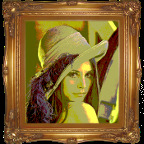
\includegraphics[width=\textwidth]{frame1}
        \caption{Originalni okvir}
    \end{subfigure}
    \begin{subfigure}[b]{0.6\textwidth}
        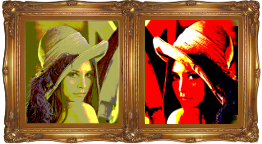
\includegraphics[width=\textwidth]{frame2}
        \caption{Novi razširjeni okvir}
        \label{fig:frame2}
    \end{subfigure}
    \caption{Prikaz razširitve okvirja zaradi menjave širšega zaslona LCD}
\end{figure}


\section{Obraz kot mozaik iz majhnih obrazov}
Prvotna instalacija ``15 sekund slave'' me je najbolj prepričala s sliko
Marilyn Monroe~\ref{fig:15sec-marilyn}, ki je sestavljena iz več
obrazov~\cite{katalog_solina}, da izgleda kot mozaik~\cite{thesisSasoStulac}.
Ker tukaj nimamo tako velike baze obrazov, smo vse skupaj malo poenostavili in
uporabili kar iste obraze, vendar obdelane z drugimi filtri. Da pa je bila
slika od daleč razločna, smo obrazu, ki je prikazan kot ``piksel'', prilili
originalno barvo\footnote{Prejšnji končni rezultat instalacije obraza smo
spremenili v sliko velikosti \textit{širina $*$ višina $=$ novo število
obrazov}.}. Ta slika (primer lahko vidimo na sliki~\ref{fig:FoF-marilyn}) je
končni prikaz naše nove instalacije.

\begin{figure}[!ht]
    \centering
    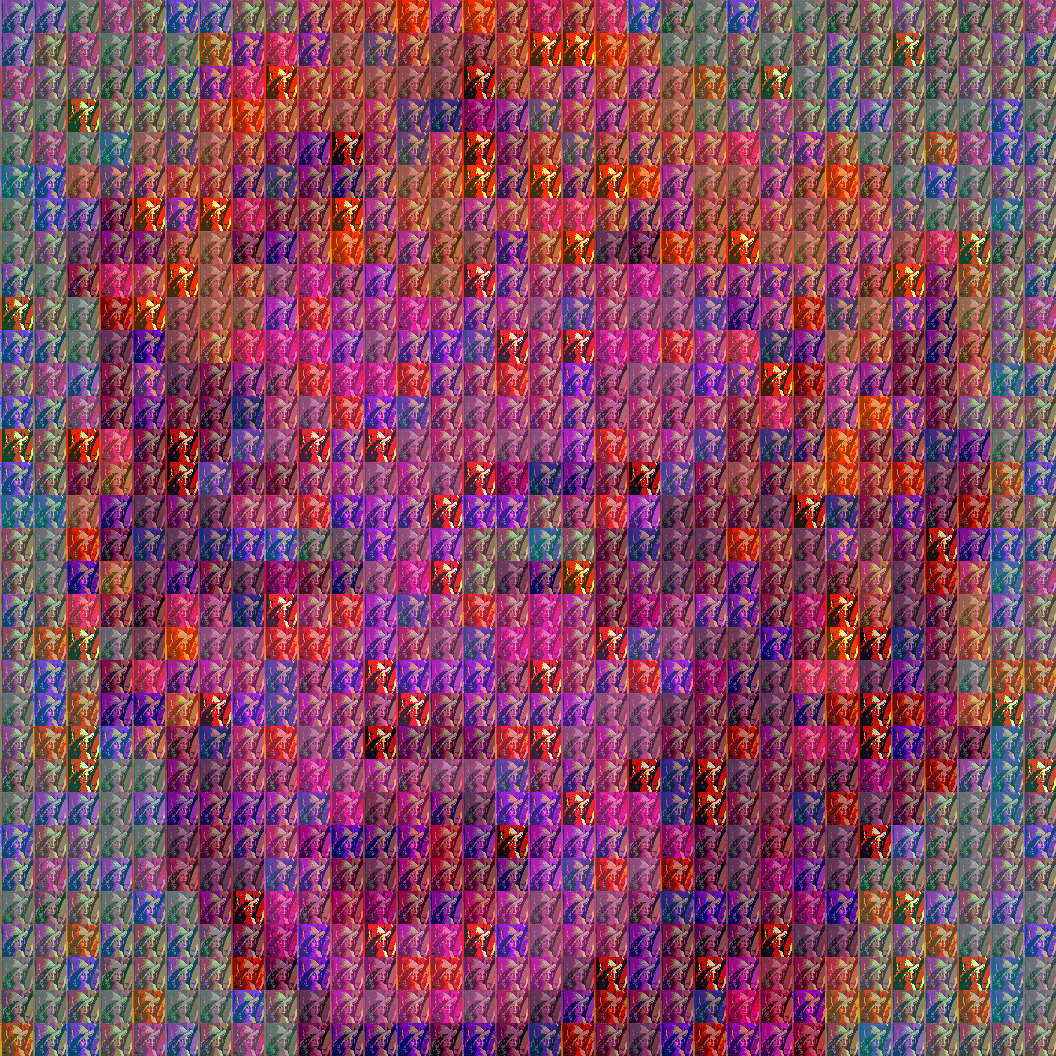
\includegraphics[width=\textwidth]{FoF-marilyn}
    \caption{Prikaz 1024 slik Lene, prikazanih na podoben način kot slika~\ref{fig:15sec-marilyn}.}
    \label{fig:FoF-marilyn}
\end{figure}


\chapter{Povezovanje s socialnimi omrežji}
\label{ch:socialNetwork}
Ena izmed pomembnejših posodobitev je povezava s socialnimi omrežji, ki so
vsak dan bolj popularna. Vsak dan se na različnih socialnih omrežjih doda na
tisoče ``selfijev''\footnote{Slika, ko oseba fotografira
samo sebe pri različnih dejavnostih.}. Da pa ta ``selfi'' še bolj pade v
oči, se jim lahko doda kakšen vnaprej določen filter. Ti so pri pametnih
telefonih, ki so danes ena izmed najpogostejših naprav za fotografiranje
``selfijev'', na voljo samo en dotik stran. Obstajajo pa tudi socialna
omrežja, ki ponujajo osnovne filtre že pri nalaganju slike.

Naša instalacija se lahko interpretira kot generator ``selfijev''. Oseba, ki
stoji pred instalacijo, ve, da bo kmalu njenih petnajst sekund. Pred njo se bo
pokazala popart slika, ki je njen umetniški ``selfi'', in če želi, je ta
popart slika lahko kmalu javno objavljena na enem izmed socialnih omrežij; lahko
se na primer dotakne ikone in tako odloči, da se njen portret prenese na želeno
socialno omrežje.

%TODO: poglej ce je potrebno
\pagebreak


\section{Možnosti}
Najpogosteje so uporabljena naslednja socialna omrežja:
\begin{description}
\item[Facebook]
Trenutno najbolj razširjeno socialno omrežje, ki ga uporabljajo vse
generacije.

\item[Twitter]
Socialno omrežje, najbolj namenjeno kratkim sporočilom, imenovanim ``tviti''.

\item[Instagram]
Socialno omrežje, predvsem namenjeno nalaganju slik. Omo\-go\-ča tudi veliko
število filtrov za obdelavo le-teh.

\item[Google+]
Alternativa socialnemu omrežju Facebook podjetja Google.

\item[Pinterest]
Socialno omrežje, predvsem namenjeno ustvarjalnostim, ki so prikazane v obliki
slik.

\item[SnapChat]
Aplikacija, ki omogoča pošiljanje slik, ki so vidne le nekaj sekund. Po
pretečenem času, to je maksimalno deset sekund~\cite{wiki:SnapChat}, slika ni
več na voljo.
\end{description}


\section{Implementacija s socialnim omrežjem Facebook}
Skoraj vsa socialna omrežja imajo omogočene javne API-je in Facebook ni nobena
izjema. Preko vmesnika API, imenovanega Graph, lahko programsko naredimo
večino akcij, ki so na voljo uporabniku preko spletnega brskalnika.

Da pa je poskrbljeno za varnost in zasebnost, je za dovoljenje uporabe Graph
API-ja potrebno narediti novo aplikacijo (\textit{angl. app}). Tu določimo,
katere pravice želimo naši aplikaciji dodeliti. Več pravic kot bomo
zahtevali, manj zaupanja vredna bo naša aplikacija, če ni uporabniku očitno,
zakaj aplikacija te pravice potrebuje. Zato je priporočljivo, da se zahtevajo
le pravice, ki jih nujno potrebujemo za delovanje naše aplikacije. V našem
primeru potrebujemo pravico, da lahko pišemo in objavljamo slike na zid
uporabnika.

Ko aplikacijo pripravimo, jo morajo uslužbenci pri podjetju Facebook
potrditi. To je varnostni postopek, brez katerega naše aplikacije ne
moremo javno uporabljati.

Ko je aplikacija narejena in potrjena, dobimo poseben ključ, ki je potreben za
povezavo z Graph API-jem. Graph API lahko uporabljamo na več načinov.
Najbolj osnoven je preko protokola HTTP, a je hkrati najbolj zahteven za
implementacijo. Drugi način je preko knjižnice, prilagojene za naprave
Android. S to knjižnico lahko na enostaven način opravimo vse osnovne akcije,
kot sta prijava v sistem in objavljanje slike.


\section{Omejitve}
Ena izmed največjih nevarnosti uporabe socialnih omrežij je nenadzorovano
pošiljanje slik na socialno omrežje. Na slikah so lahko osebe, ki si ne želijo
biti objavljene na socialnem omrežju, saj je javno. Še več, na slikah so lahko
otroci, katerih objavljanje slik na socialnem omrežju je brez dovoljenja
staršev prepovedano. Res je, da smo želeli slike izbrisati petnajst sekund po
objavi, vendar pa večina socialnih omrežjih te slike še vedno hrani, čeprav
jih ne vidimo več. In če se podamo še v najhujšo skrajnost, nekdo bi lahko
napisal program, ki vse slike shranjuje na nek strežnik, in bi nato z njimi
razpolagal po svoji volji.


\chapter{Sklepne ugotovitve}
V sklopu magistrske naloge smo posodobili strojno in programsko opremo
instalacije ``15 sekund slave''. Razvoj novih uporabnih funkcionalnosti nam je
omogočil, da smo instalaciji dodali tudi nekaj novih možnosti, ki naredijo
uporabniško izkušnjo še bolj zanimivo.

Digitalni fotoaparat in osebni računalnik smo zamenjali s pametnim telefonom,
s čimer smo dosegli, da instalacija zavzame manj prostora, saj je uporabljenih
manj komponent, kot jih je bilo prej, poleg tega pa je omogočeno tudi lažje
vzdrževanje in odpravljanje morebitnih napak, saj se vse nahaja na eni
napravi.

S posodobitvijo programske opreme smo omogočili, da instalacija deluje na eni
napravi in dodali nove funkcionalnosti:
\begin{itemize}
    \item povezovanje s socialnimi omrežji, kar je predvsem za mlajše uporabnike zaželena prednost;
    \item sestavljanje končnega obraza iz več obrazov, ki so obdelani z različnimi filtri;
    \item posodobitev in optimizacija algoritmov za filtriranje slik;
    \item posodobitev in optimizacija algoritmov za zaznavanje obrazov.
\end{itemize}

V prihodnosti obstaja možnost, da se filtri uporabijo tudi v drugih
aplikacijah, saj so filtri napisani kot knjižnica, uporaba te pa je
enostavna. Predstavljajmo si aplikacijo, kot je Instagram, ki ima tudi
možnost popart filtrov, napisanih v tej magistrski nalogi.

Poleg tega bo potrebno redno vzdrževanje instalacije, tako na
nivoju strojne opreme kot tudi na nivoju programske opreme, saj želimo ostati
v koraku s časom.

Med izvedbo naloge smo se večkrat soočili z vprašanjem, do kakšne mere
instalacijo še lahko spreminjamo, da umetnina še vedno ostane ista in ne nekaj
povsem novega. Na tem področju se je tudi pojavilo največ težav. Čeprav je na
prvi pogled le enostavna ponovna implementacija že narejene instalacije, pa
vendar pri umetniškem delu ni vse samo v programu. Zelo veliko pozornosti
moramo namreč nameniti temu, da umetnina za opazovalca ostane taka, kot je
bila.





%----------------------------------------------------------------
% SLO: bibliografija
% ENG: bibliography
%----------------------------------------------------------------
\bibliographystyle{elsarticle-num}
% \bibliography{bibliography} HARDCODED!!!

\begin{thebibliography}{99}
\bibitem{firstdecade}
F.~Dietrich, ``Visual intelligence: the first decade of computer art (1965--1975)'', \textit{Leonardo}, zv. 19, št. 2, str. 159--169, 1968.

\bibitem{thesisSamoJuvan}
S.~Juvan, ``Predelava fotografij z barvnimi filtri v slogu pop-art'', Diplomsko delo, Fakulteta za računalništvo in informatiko, Univerza v Ljubljani, 2002.

\bibitem{kovac2003illumination} J.~Kovač, P.~Peer, F.~Solina, ``Illumination independent color-based face detection'', v \textit{Proceedings of the 3rd International Symposium on Image and Signal Processing and Analysis (ISPA 2003)}, IEEE, zv. 1, str. 510--515, 2003.

\bibitem{lieser2010world}
W.~Lieser, ``The World of Digital Art'', h.f. Ullmann, 2010.

\bibitem{miller2}
P.~Miller, ``Technology for art's sake'', \textit{IEEE Spectrum}, zv. 35, št. 7, str. 30--37, 1998.

\bibitem{miller1}
P.~Miller, ``The engineer as catalyst: Billy Kl\"{u}ver on working with artists'', \textit{IEEE Spectrum}, zv. 35, št. 7, str. 20--29, 1998.

\bibitem{nevenFaceRecognition}
P.~J. Phillips, W.~T. Scruggs, A.~J. O’Toole, K.~W. Bowyer, P.~J. Flynn, C.~L. Schott, M.~Sharpe, ``Frvt 2006 and ice 2006 large-scale experimental results'', \textit{Pattern Analysis and Machine Intelligence, IEEE Transactions on}, zv. 32, št. 5, str. 831--846, 2010.

\bibitem{ZKM}
B.~Serexhe, ur., \textit{Preservation of Digital Art: Theory in Praxis}. Karlsruhe: AMBRA $|$ V, ZKM $|$ Center for Art in Media, 2013.

\bibitem{AW}
J.~B. Simpson, ``Simpson's contemporary quotations: The most notable quotes from 1950 to the present''. HarperCollins Publishers, 1997.

\bibitem{leonardo}
F.~Solina, ``15 seconds of fame'', \textit{Leonardo}, zv. 37, št. 2, str. 105--110, 2004.

\bibitem{katalog_solina}
F.~Solina, \textit{15 sekund slave in virtualno smučanje / 15 Seconds of Fame and Virtual Skiing. Exhibition Catalogue}. Ljubljana: ArtNetLab, 2005.

\bibitem{mirage03}
F.~Solina, B.~Batagelj, S.~Juvan, J.~Kovačič, ``Color-based face detection in the ``15 seconds of fame'' art installation'', v \textit{Proceedings of Mirage 2003}, NRIA Rocquencourt, Francija, str. 38--47, 2003.

\bibitem{preservationComputerBasedArt}
F.~Solina, G.~Majcen, N.~Bovcon, B.~Batagelj, ``Preservation of a computer-based art installation'', \textit{EuroMed 2014}, str. 643--650, 2014.

\bibitem{solina200215}
F.~Solina, P.~Peer, B.~Batagelj, S.~Juvan, ``15 seconds of fame-an interactive, computer---vision based art installation'', v \textit{Proc. 7th International Conference on Control, Automation, Robotics and Vision}, IEEE, zv. 1, str. 198--204, 2002.

\bibitem{trifonova}
A.~Trifonova, L.~Jaccheri, K.~Bergaust, ``Software engineering issues in interactive installation art'', \textit{International Journal of Arts and Technology}, zv. 1, št. 1, str. 43--65, 2008.

\bibitem{viola2004robust}
P.~Viola, M.~J. Jones, ``Robust real-time face detection'', \textit{International journal of computer vision}, zv. 57, št. 2, str. 137--154, 2004.

\bibitem{thesisSasoStulac}
S.~Štulac, ``Samodejna gradnja mozaika'', Diplomsko delo, Fakulteta za računalništvo in informatiko, Univerza v Ljubljani, 2008.

\bibitem{andyExhibitionMonroe}
A.~Warhol, ``Marilyn Monroe'', \textit{Collection of The Andy Warhol Museum, Pittsburgh}, 1967.

\bibitem{andyExhibition}
A.~Warhol, ``Andy Warhol, Exhibition catalogue'', \textit{Moderna Museet, Stockholm}, 1968.

\bibitem{wiki:Android}
Wikipedia, \textit{Android --- Wikipedia, The Free Encyclopedia}, [zadnji obisk 26.04.2015], 2015. Dostopno na: \url{https://en.wikipedia.org/wiki/Android_(operating_system}

\bibitem{wiki:AndyWarhol}
Wikipedia, \textit{Andy Warhol --- Wikipedia, The Free Encyclopedia}, [zadnji obisk 26.04.2015], 2015. Dostopno na: \url{https://en.wikipedia.org/wiki/Andy_Warhol}

\bibitem{wiki:GIMP}
Wikipedia, \textit{GIMP --- Wikipedia, The Free Encyclopedia}, [zadnji obisk 26.04.2015], 2015. Dostopno na: \url{https://en.wikipedia.org/wiki/GIMP}

\bibitem{wiki:SnapChat}
Wikipedia, \textit{Snapchat --- Wikipedia, The Free Encyclopedia}, [zadnji obisk 26.04.2015], 2015. Dostopno na: \url{https://en.wikipedia.org/wiki/Snapchat}
\end{thebibliography}



\backmatter
\end{document}
